\documentclass[openany]{mitthesis}

% Encoding and Language Settings
\usepackage[utf8]{inputenc}       % Enables UTF-8 encoding
\usepackage[T5]{fontenc}          % Supports Vietnamese characters
\usepackage[english]{babel}       % Language support (can change to [vietnamese])

% Typography and Font Settings
\usepackage{lmodern}
\usepackage[protrusion=true, expansion=false]{microtype}
\usepackage{ragged2e} % Provides the \RaggedRight command

\usepackage{neuralnetwork}

% Math and Theorem Environments
\usepackage{amsmath, amssymb, amsthm, bm}
\usepackage{mathtools}
\DeclareMathOperator{\Erf}{erf}
\DeclareMathOperator{\Erfc}{erfc}
\DeclarePairedDelimiterXPP\erf[1]{\Erf\mkern1mu}(){}{#1}
\DeclarePairedDelimiterXPP\erfc[1]{\Erfc\mkern1mu}(){}{#1}

% Theorem Styles
\newtheorem{theorem}{{\bf Theorem}}
\newtheorem{property}{{\bf Property}}
\newtheorem{proposition}{{\bf Proposition}}
\newtheorem{corollary}[proposition]{{\bf Corollary}}
\newtheorem{lemma}[proposition]{{\bf Lemma}}
\theoremstyle{definition}
\newtheorem{definition}{Definition}[section]

% Graphics and Colors
\usepackage{graphicx, tikz}
\usetikzlibrary{arrows, snakes, backgrounds, patterns, shapes, calc, positioning, matrix, fit}
\usepackage{pgfplots}
\usepackage{xcolor}
\definecolor{gray}{RGB}{247, 247, 247}
\definecolor{pr}{RGB}{0, 32, 128}
\definecolor{codegreen}{rgb}{0,0.6,0}
\definecolor{codepurple}{rgb}{0.58,0,0.82}
\definecolor{backcolour}{rgb}{0.95,0.95,0.92}

\usepackage{csquotes}

% Code Listings
\usepackage{listings}
\lstdefinestyle{mystyle}{
  backgroundcolor=\color{backcolour}, commentstyle=\color{codegreen},
  keywordstyle=\color{magenta}, numberstyle=\tiny\color{gray},
  stringstyle=\color{codepurple}, basicstyle=\ttfamily\footnotesize,
  breaklines=true, numbers=left, numbersep=5pt, tabsize=2
}
\lstset{style=mystyle}

% Tables
\usepackage{array, tabularx, booktabs, longtable, multirow, adjustbox, caption}
\usepackage{dcolumn}
\newcolumntype{d}[1]{D{.}{.}{#1}}

% Algorithm and Pseudocode
\usepackage{algorithm}
\usepackage{algpseudocode}

% Hyperlinks and References
\usepackage{hyperref}
\usepackage{bookmark}
\hypersetup{
  colorlinks=true,
  linktoc=all,
  linkcolor=blue,
  citecolor=black,
  urlcolor=black,
  pdfsubject={MIT Thesis Template with Added Features},
  % pdfkeywords={Massachusetts Institute of Technology, MIT},
  pdfkeywords={Ho Chi Minh City University of Technology, MIT},
  pdfauthortitle={}
}

% Fancy Header and Footer
\usepackage{fancyhdr, lastpage}

% Markdown Support
\usepackage[fencedCode,citations,definitionLists,hashEnumerators,smartEllipses,pipeTables,tableCaptions,hybrid]{markdown}

% Section Depth Configuration
\setcounter{secnumdepth}{4}
\setcounter{tocdepth}{4}
\makeatletter
\newcounter{subsubsubsection}[subsubsection]
\renewcommand\thesubsubsubsection{\thesubsubsection.\@alph\c@subsubsubsection}
\newcommand\subsubsubsection{\@startsection{subsubsubsection}{4}{\z@}%
                                     {-3.25ex\@plus -1ex \@minus -.2ex}%
                                     {1.5ex \@plus .2ex}%
                                     {\normalfont\normalsize\bfseries}}
\makeatother

% Custom Commands and Boxes
\newcommand*\circled[1]{\tikz[baseline=(char.base)]{
    \node[shape=circle,draw,inner sep=0.1pt] (char) {#1};}}

\usepackage[most]{tcolorbox}
\newtcolorbox{cmt}[1]{
  boxrule=0pt, boxsep=0pt, colback=gray,
  detach title, before upper={\tcbtitle \ },
  fonttitle=\bfseries\sffamily, coltitle=pr, title=#1,
  borderline west={2.5pt}{0pt}{pr}, enhanced jigsaw,
  before skip=10pt, after skip=10pt, breakable
}

\newcommand{\myItemize}[1]{%
    \begin{itemize}
        #1
    \end{itemize}
}

\usepackage{forest}

%%%%%%%%%%% Bibliography %%%%%%%%%%%%
\usepackage[style=ext-numeric-comp,giveninits=true,maxbibnames=10,sorting=none]{biblatex}
\addbibresource{references.bib}

\setlength{\parskip}{0.5em}       % Paragraph spacing
\setlength{\parindent}{0pt}       % Disable paragraph indentation

\begin{document}

%%% edit the following commands to match your thesis %%%%%%%%%%

\begin{titlepage}
% Temporarily adjust margins for this page only
\newgeometry{top=2cm, bottom=4cm, left=2cm, right=2.5cm} % Adjust as needed
\begin{center}
VIETNAM NATIONAL UNIVERSITY, HO CHI MINH CITY \\
UNIVERSITY OF TECHNOLOGY \\
FACULTY OF COMPUTER SCIENCE AND ENGINEERING
\end{center}

\begin{figure}[h!]
\begin{center}

\includegraphics[width=6cm]{hcmut.png}
\end{center}
\end{figure}

\begin{center}
\begin{tabular}{c}
\multicolumn{1}{l}{\textbf{{\Large NATURAL LANGUAGE PROCESSING (CO3086)}}}\\
~~\\
\hline
\\
\multicolumn{1}{l}{\textbf{{\Large Assignment:}}}\\
\\
\textbf{{\Huge Transformer and Applications}}\\
\\
\textbf{{\Huge}}\\
\\
\hline
\end{tabular}
\end{center}

\vspace{1cm}

\begin{table}[h]
\begin{tabular}{rrll}
\hspace{5 cm} & Advisor: & Bui Khanh Vinh & \\
& Students: & Thai Quang Phat &- 2252606 (\textbf{Leader}) \\
& & Nguyen Quang Phu &- 2252621 (Member) \\
& & Nguyen Tien  Hung &- 2252280 (Member) \\
& & Nguyen Ngoc Khoi &- 2252378 (Member) \\
& & Tran Nguyen The Nhat &- 2252556 (Member) \\
\end{tabular}
\end{table}

\begin{center}
{\footnotesize HO CHI MINH CITY, MAY 2025}
\end{center}
\restoregeometry
\end{titlepage}

\tableofcontents
\listoffigures
\listoftables

\pgfplotsset{compat=1.18}

% % %%%%%%%%%%%%%%%%%%%%%%%%%%%%%%%%%%%%%%%%%%

\chapter{Abstract}

The rapid advancement of Transformer-based Large Language Models (LLMs) has revolutionized Natural Language Processing (NLP), enabling significant improvements in tasks such as text generation, machine translation, and text summarization. However, the exponential growth in model size and complexity has introduced challenges in adapting these models efficiently for task-specific applications.

This project focuses on exploring and analyzing fine-tuning techniques that optimize large Transformer-based models while reducing computational cost. By applying different fine-tuning strategies, including full fine-tuning, adapter-based methods, and parameter-efficient fine-tuning (PEFT) approaches such as LoRA and prompt tuning, we aim to evaluate their effectiveness across multiple NLP tasks. 

Through rigorous experimentation, we assess the trade-offs between computational efficiency and model performance, providing insights into the best practices for fine-tuning LLMs in real-world applications. The findings contribute to advancing research in optimizing Transformer-based models for task-specific deployment while addressing scalability challenges.

\newpage

\chapter{Description}

Since 2017, the introduction of the Transformer model has significantly transformed the field of Natural Language Processing (NLP). The Transformer architecture, proposed by Vaswani et al. in the paper \textbf{``Attention Is All You Need''}, replaced traditional recurrent and convolutional networks with self-attention mechanisms. This innovation enabled efficient parallel computation, resulting in improved training speed and model performance.

Transformers have since become the foundation of state-of-the-art NLP models such as \textbf{BERT}, \textbf{GPT}, and \textbf{T5}. These models leverage massive datasets and billions to trillions of parameters, leading to breakthroughs in various NLP tasks. However, the increasing scale of LLMs has also introduced challenges related to computational efficiency, making full fine-tuning infeasible in many scenarios.

To address these challenges, researchers have developed various fine-tuning techniques that balance efficiency and performance. Parameter-efficient fine-tuning (PEFT) methods such as LoRA, adapter-based fine-tuning, and prompt tuning allow practitioners to adapt large models with minimal computational overhead. These approaches enable LLMs to be utilized in domain-specific applications while mitigating the resource constraints typically associated with full fine-tuning.

This study investigates the development and fine-tuning of Transformer-based models, examining their evolution, key milestones, and experimental applications. By evaluating different fine-tuning strategies, we aim to provide insights into how LLMs can be optimized for real-world NLP tasks without excessive computational requirements.

\newpage
\chapter{Transformer Models}

\section{Overview of Transformer Model}

The Transformer model is a major breakthrough in machine learning, particularly in \textbf{Natural Language Processing (NLP)}. Introduced by Vaswani et al. in 2017 with the paper \textit{“Attention is All You Need”}, it replaced traditional recurrence-based architectures with \textbf{self-attention mechanisms}, enabling state-of-the-art performance and improved scalability.

Prior to Transformers, sequence models relied on \textbf{Recurrent Neural Networks (RNNs)}, such as \textbf{LSTMs} and \textbf{GRUs}, which processed inputs sequentially. However, they struggled with long-range dependencies, slow training due to sequential processing, and limited parallelization. Convolutional models improved efficiency but failed to capture global dependencies effectively.

The Transformer addressed these issues with \textbf{self-attention}, allowing each token to attend to all others simultaneously, eliminating sequential dependencies and enabling full parallelization. Additional innovations include \textbf{multi-head attention} for learning diverse relationships, \textbf{positional encoding} to retain order, and \textbf{feed-forward networks (FFN)} for feature transformation, along with \textbf{residual connections and layer normalization} for stable training.

Initially designed for \textbf{sequence-to-sequence tasks} like machine translation, Transformers have since revolutionized multiple domains. Models like \textbf{BERT, GPT, and T5} dominate NLP tasks, while \textbf{Vision Transformers (ViTs)} challenge CNNs in computer vision. Transformers also play a crucial role in \textbf{speech processing, multimodal learning, reinforcement learning}, and \textbf{robotics}, demonstrating their versatility.

As research continues, advancements such as \textbf{sparse attention} and \textbf{memory-efficient architectures} further enhance Transformer capabilities. With its scalability and adaptability, the Transformer remains a cornerstone of modern AI, shaping the future of deep learning.

\newpage

\section{Transformer Architecture in Detail}

The Transformer architecture, introduced in \textit{Attention Is All You Need} (Vaswani et al., 2017), is a modular and scalable design that has revolutionized sequence modeling by forgoing recurrence and convolutions in favor of a purely attention-based mechanism. Its foundational elements include tokenization, embedding, self-attention, multi-head attention, positional encoding, encoder-decoder stacks, and un-embedding layers.

\begin{figure}[H]
    \centering
    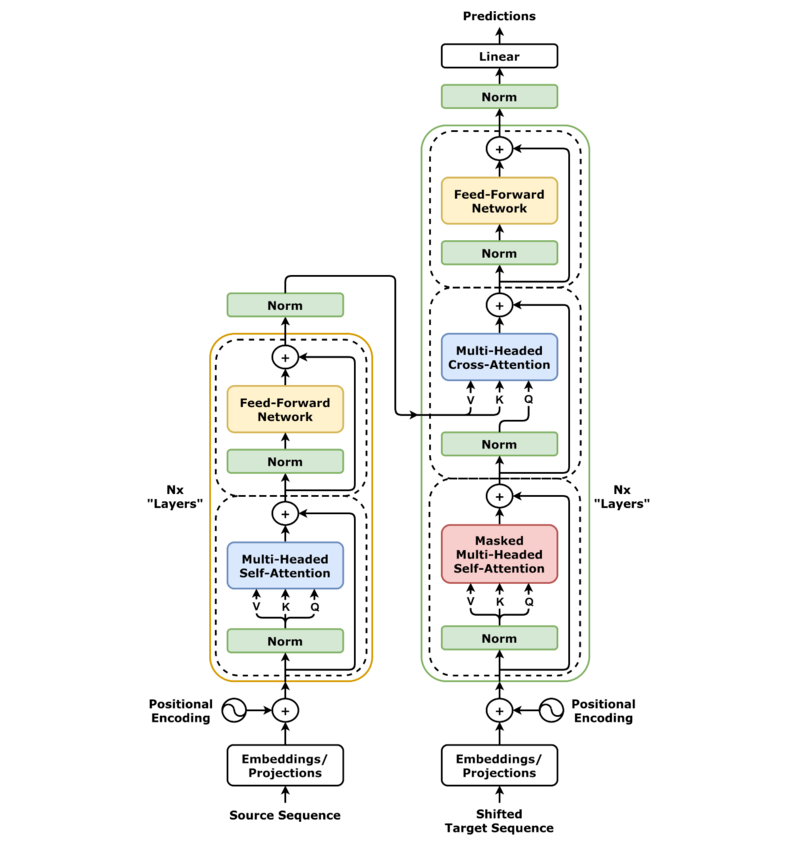
\includegraphics[width=\textwidth]{img/chap03/Transformer_architecture.png} % Adjust width as needed
    \caption{Transformer Encoder-Decoder Architecture}
    \label{fig:transformer_architecture}
\end{figure}

\subsection{Tokenization}

Before text is processed by the Transformer, it must be converted into tokens. A \textbf{tokenizer} maps segments of text (such as words, subwords, or characters) into integers from a finite vocabulary $V$ of size $n_{\text{vocab}}$. Examples of tokenization methods include Byte-Pair Encoding (BPE), WordPiece, and SentencePiece.

The input text is transformed into a token sequence:
\[
\text{``The dog barks''} \rightarrow [101, 1996, 3899, 3985, 102]
\]

Here, 101 and 102 may represent special start and end tokens.

\subsection{Embedding Layer}

The first step in a Transformer is to convert discrete token indices into continuous vector representations. This is done through a learnable \textbf{embedding layer}, which uses an embedding matrix $E \in \mathbb{R}^{n_{\text{vocab}} \times d_{\text{model}}}$, where:

\begin{itemize}
  \item $n_{\text{vocab}}$ is the size of the vocabulary,
  \item $d_{\text{model}}$ is the model dimensionality.
\end{itemize}

Each token index $t_i$ is mapped to its corresponding vector via lookup in $E$:

\[
\text{Embed}(t_i) = E[t_i] \in \mathbb{R}^{d_{\text{model}}}
\]

This can be interpreted as multiplying a one-hot vector $\mathbf{1}_{t_i} \in \mathbb{R}^{n_{\text{vocab}}}$ by the embedding matrix:

\[
\text{Embed}(t_i) = \mathbf{1}_{t_i}^\top E
\]

Embedding vectors serve as the input to the model and are updated during training to capture semantic relationships between tokens.

\subsection{Un-Embedding Layer}

At the output of the decoder (in encoder-decoder models) or the model head (in decoder-only models), we obtain hidden vectors $x \in \mathbb{R}^{d_{\text{model}}}$, which must be transformed back into the vocabulary space to compute probabilities over possible next tokens.

This is done using an \textbf{un-embedding layer}, also called the output projection layer, with weight matrix $W \in \mathbb{R}^{d_{\text{model}} \times n_{\text{vocab}}}$ and optional bias vector $b \in \mathbb{R}^{n_{\text{vocab}}}$:

\[
\text{UnEmbed}(x) = \text{softmax}(xW + b)
\]

The result is a probability distribution over all tokens in the vocabulary. Many modern Transformer implementations apply \textbf{weight tying}, where the output matrix $W$ is tied to the input embedding matrix $E$:

\[
W = E^\top
\]

This reduces the number of parameters and can improve generalization, as input and output embeddings share a common representation space.

\subsection{Positional Encoding}

Transformers process input embeddings in a permutation-invariant manner, lacking inherent order information. To encode token positions, a \textbf{positional encoding} vector is added:

\[
x_i = \text{Embed}(t_i) + \text{PosEnc}(i)
\]

where $\text{PosEnc}(i) \in \mathbb{R}^{d_{\text{model}}}$ represents the positional encoding at position $i$.

${}$\\
\textbf{Sinusoidal Positional Encoding}

The Transformer model uses a fixed sinusoidal function:

\[
\text{PosEnc}(i)_{2k} = \sin\left(\frac{i}{10000^{\frac{2k}{d_{\text{model}}}}}\right), \quad
\text{PosEnc}(i)_{2k+1} = \cos\left(\frac{i}{10000^{\frac{2k}{d_{\text{model}}}}}\right)
\]

ensuring unique encodings, relative position awareness, and generalization to unseen sequences.

${}$\\
\textbf{Complex Representation and Shift Property}

A compact formulation uses complex numbers:

\[
f(t) = \left( e^{i t / r^k} \right)_{k=0,1,\dots,d/2 -1}, \quad r = N^{2/d}
\]

where $N = 10000$. A key property is shift linearity:

\[
f(t + \Delta t) = \text{diag}(f(\Delta t)) f(t)
\]

allowing efficient matrix-based position updates.

${}$\\
\textbf{Implementation in Real-Valued Space}

Euler’s formula relates this to sine and cosine:

\[
e^{i x} = \cos x + i \sin x
\]

making real-number implementations straightforward.

${}$\\
\textbf{Example: Encoding in a 16D Space}

For $d_{\text{model}} = 16$ and $t=5$, resulting in a 16D vector:

\[
\text{PosEnc}(5)_{2k} = \sin\left(\frac{5}{10000^{2k/16}}\right), \quad
\text{PosEnc}(5)_{2k+1} = \cos\left(\frac{5}{10000^{2k/16}}\right)
\]

\subsection{Self-Attention Mechanism}

Each input vector is linearly projected into three spaces: queries $Q$, keys $K$, and values $V$:
\[
Q = XW^Q, \quad K = XW^K, \quad V = XW^V
\]

The attention weights between tokens are computed using the scaled dot-product attention:
\[
\text{Attention}(Q, K, V) = \text{softmax} \left( \frac{QK^\top}{\sqrt{d_k}} \right)V
\]

This allows the model to dynamically attend to relevant tokens within the sequence.

\subsection{Multi-Head Attention}

In Transformers, a single attention mechanism may not be sufficient to capture different relationships in the input sequence. Instead of computing attention once, the model employs multiple \textbf{attention heads}, each with its own set of projection matrices:

\[
\text{head}_i = \text{Attention}(QW_i^Q, KW_i^K, VW_i^V)
\]

where each head $i$ independently projects queries, keys, and values using learned weight matrices $W_i^Q$, $W_i^K$, and $W_i^V$.

Outputs of all attention heads are concatenated, projected using final output matrix $W^O$:

\[
\text{MultiHead}(Q, K, V) = \text{Concat} \left( \text{head}_1, \dots, \text{head}_{h} \right) W^O
\]

where:
\begin{itemize}
    \item $h$ is the number of attention heads.
    \item Each head learns a different attention pattern, allowing the model to attend to multiple aspects of the input.
    \item The final projection matrix $W^O$ ensures that the multi-head attention output remains in the original embedding space.
\end{itemize}

\begin{figure}[H]
    \centering
    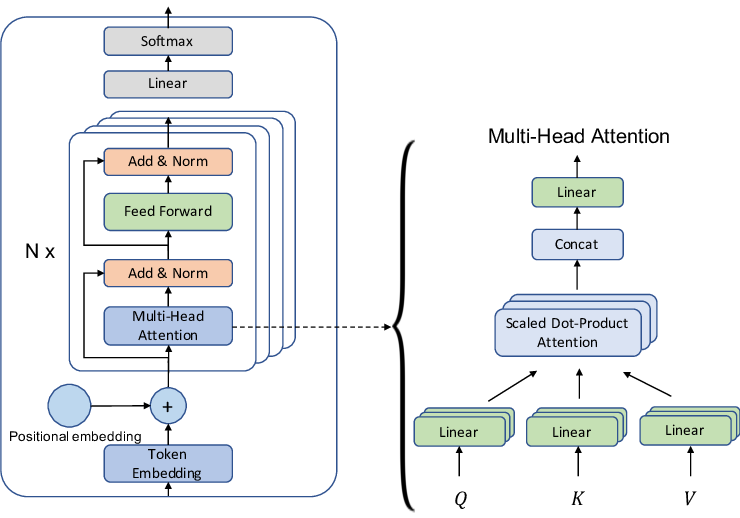
\includegraphics[width=0.7\textwidth]{img/chap03/Multiheaded.png} 
    \caption{Multiheaded attention}
    \label{fig:multi-head-attention}
\end{figure}

In practice, the embedding dimension $d_{\text{model}}$ is split across $h$ heads, with each head operating on a subspace of size $d_{\text{head}} = d_{\text{model}} / h$. For example, in GPT-2 Small:

\[
d_{\text{model}} = 768, \quad n_{\text{head}} = 12, \quad d_{\text{head}} = 64
\]

Since $12 \times 64 = 768$, the output projection matrix $W^O$ has dimensions:

\[
W^O \in \mathbb{R}^{(12 \times 64) \times 768}
\]

which ensures that the output dimension remains consistent.

This mechanism allows the Transformer to capture both local and global dependencies across different attention heads in parallel, improving expressiveness and performance.

\subsection{Feedforward Network (FFN)}

Each encoder and decoder layer contains a position-wise FFN applied independently:
\[
\text{FFN}(x) = \phi(xW^{(1)} + b^{(1)})W^{(2)} + b^{(2)}
\]
where $\phi$ is a non-linearity such as ReLU or GELU. Typically, $d_{\text{ff}} = 4d_{\text{model}}$.

\begin{figure}[H]
    \centering
    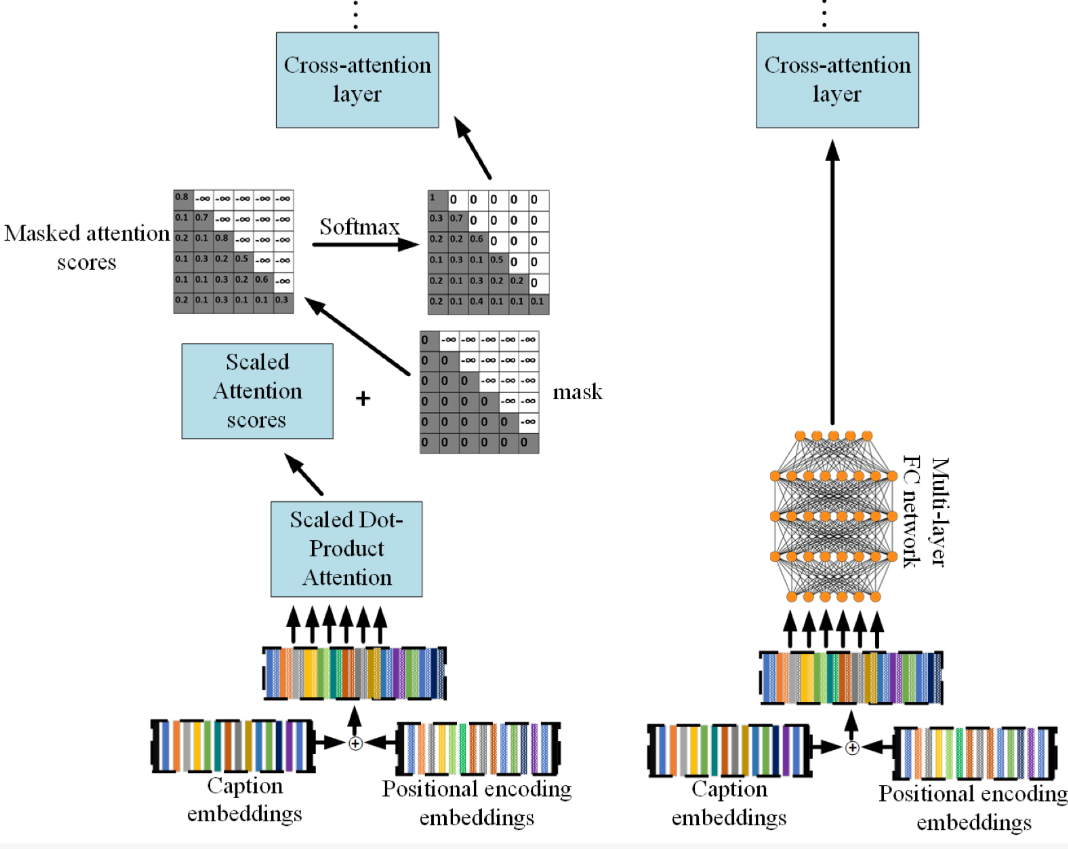
\includegraphics[width=\textwidth]{img/chap03/feed-forward.PNG} 
    \caption{The Use of Feed-Forward for Transformer Based Image Captioning Tasks}
    \label{fig:feed-forward}
\end{figure}

The figure illustrates the use of FFN and masked attention in image captioning. The left side depicts \textbf{masked attention}, where embeddings undergo scaled dot-product attention with a causal mask to maintain autoregressive properties. On the right, the \textbf{feed-forward network} refines the attended representations through a multi-layer transformation before passing them to the cross-attention layer. This enhances feature extraction and enables richer caption generation.

\subsection{Residual Connections and Layer Normalization}

Every sublayer (attention or FFN) is surrounded by a residual connection and followed (or preceded) by layer normalization (LayerNorm). Two conventions exist:

\begin{itemize}
    \item \textbf{Post-LN}: $\text{LayerNorm}(x + \text{Sublayer}(x))$
    \item \textbf{Pre-LN}: $x + \text{Sublayer}(\text{LayerNorm}(x))$
\end{itemize}

Pre-LN has been shown to stabilize training and eliminate need for learning rate warm-up.

\subsection{Encoder and Decoder Structure}

\textbf{Encoder:}

Each encoder block consists of:
\begin{enumerate}
    \item Multi-head self-attention
    \item Feed-forward network
\end{enumerate}

Each layer processes the entire sequence simultaneously using all-to-all attention.

\textbf{Decoder:}

Each decoder block consists of:
\begin{enumerate}
    \item Masked multi-head self-attention (causal)
    \item Cross-attention (to encoder outputs)
    \item Feed-forward network
\end{enumerate}

Masked attention ensures that future tokens are not visible during training.

\subsection{Masked Attention}

In Transformer decoders, masked attention ensures autoregressive token generation by preventing each token from attending to future tokens. This is achieved by adding a mask matrix $M$, which assigns $-\infty$ to positions that should not be attended to, ensuring causality before applying the softmax operation:

\[
\text{MaskedAttention}(Q, K, V) = \text{softmax} \left( M + \frac{QK^\top}{\sqrt{d_k}} \right) V
\]

where:
\begin{itemize}
    \item $Q, K, V$ are the query, key, and value matrices.
    \item $d_k$ is the key dimension.
    \item $M$ is a lower triangular matrix that blocks future tokens.
\end{itemize}

The commonly used \textbf{causal mask} is defined as:

\[
M_{\text{causal}} =
\begin{bmatrix}
0 & -\infty & -\infty & \cdots & -\infty \\
0 & 0 & -\infty & \cdots & -\infty \\
0 & 0 & 0 & \cdots & -\infty \\
\vdots & \vdots & \vdots & \ddots & -\infty \\
0 & 0 & 0 & \cdots & 0
\end{bmatrix}
\]

This mask ensures that each token can only attend to itself and past tokens, preventing information leakage from future tokens. In a non-masked attention module, $M$ is simply a matrix of zeros.

\section{Transformer Variants}

Transformers have evolved into several architectural variants, each designed for specific tasks and optimization strategies:

\begin{itemize}
    \item \textbf{Encoder-Only Models}: These architectures process the entire input sequence simultaneously, making them well-suited for tasks such as \textbf{sentence classification, named entity recognition (NER), and embedding generation}. The bidirectional nature of the encoder enables a holistic understanding of context. A prime example is \textbf{BERT}, which learns contextual representations by predicting masked tokens.
    
    \item \textbf{Decoder-Only Models}: Designed for \textbf{autoregressive generation}, these models generate tokens sequentially, conditioning each new token on previously generated ones. They are extensively used in \textbf{text generation, dialogue systems, and code synthesis}. The most prominent example is \textbf{GPT}, where decoding follows a causal attention pattern to prevent information leakage from future tokens.

    \item \textbf{Encoder-Decoder Models}: Also known as \textbf{sequence-to-sequence (seq2seq)} architectures, these models encode an input sequence into a latent representation and decode it into an output sequence. This structure is particularly effective for \textbf{machine translation, abstractive summarization, and speech-to-text conversion}. Notable examples include \textbf{T5} and \textbf{BART}, where pretraining strategies such as denoising and span prediction improve performance.

    \item \textbf{PrefixLM Models}: A hybrid approach that extends decoder-only architectures by introducing a \textbf{prefix-based masking strategy}, where certain tokens (prefix) attend to all positions while others follow causal masking. This allows for improved \textbf{controlled text generation, fill-in-the-middle tasks, and dialogue modeling}. Models like \textbf{T5 (with prefix tuning)} and \textbf{GPT-like architectures with prefix constraints} leverage this setup.
\end{itemize}

\section{Training and Pretraining Paradigms}

The effectiveness of Transformer models stems from large-scale \textbf{self-supervised pretraining}, followed by \textbf{task-specific fine-tuning}. Pretraining objectives vary based on the architecture:

\begin{itemize}
    \item \textbf{Masked Language Modeling (MLM)}: Used primarily in bidirectional encoder models like \textbf{BERT} and \textbf{RoBERTa}. In MLM, a percentage of input tokens are randomly masked, and the model is trained to predict these missing tokens based on surrounding context. This enables the model to learn deep bidirectional representations.

    \item \textbf{Autoregressive Language Modeling (AR)}: Used in decoder-only models such as \textbf{GPT}. Here, the model generates tokens sequentially, predicting the next token based on previous tokens. The training follows a left-to-right causal dependency, making it well-suited for open-ended text generation.

    \item \textbf{Prefix Language Modeling (PrefixLM)}: A hybrid approach used in models like \textbf{T5}, where a portion of the input sequence (prefix) is given full attention while subsequent tokens follow autoregressive constraints. This allows for both bidirectional understanding and controlled generation, making it useful for multitask learning.

\end{itemize}

After pretraining, these models are fine-tuned on labeled datasets for \textbf{downstream tasks} such as sentiment analysis, question answering (QA), summarization, and code generation. The fine-tuning stage involves updating model weights on task-specific objectives, often leveraging transfer learning to achieve state-of-the-art performance with limited labeled data.

\section{Advantages and Applications}

Transformers offer several advantages over previous architectures:

\begin{itemize}
    \item \textbf{No Recurrence}: Unlike RNNs or LSTMs, Transformers process input sequences in parallel, leading to faster training and inference.
    
    \item \textbf{Long-Range Dependency Modeling}: The self-attention mechanism allows direct interactions between all tokens, making it easier to capture long-range relationships.

    \item \textbf{Scalability}: Transformers can be scaled to billions of parameters and trained on large datasets across distributed systems.

    \item \textbf{Transferability}: Pretrained models serve as general-purpose language encoders and can be adapted to a wide variety of downstream tasks with minimal training data.

    \item \textbf{Multimodal Extension}: The architecture has been adapted for images (Vision Transformers), audio (e.g., Whisper), and multimodal inputs (e.g., CLIP, Flamingo).
\end{itemize}

\newpage

\section{Impacts on Natural Language Processing}

The introduction of Transformer models has profoundly transformed the field of \textbf{Natural Language Processing (NLP)}. By replacing recurrence-based architectures with self-attention mechanisms, Transformers have driven major advancements in language understanding, text generation, and multi-modal learning. Their impact extends across multiple dimensions, revolutionizing both research and real-world applications.

\subsection{Emergence of Pretrained Language Models}

Transformer-based architectures laid the foundation for a new era of \textbf{pretrained language models}, where large-scale self-supervised learning followed by task-specific fine-tuning became the dominant paradigm. Pretrained Transformers learn rich representations from massive text corpora and transfer this knowledge to a wide range of NLP tasks.

\begin{itemize}
    \item \textbf{BERT (Bidirectional Encoder Representations from Transformers)} introduced bidirectional attention, allowing models to learn deep contextual representations. Pretraining tasks such as \textbf{Masked Language Modeling (MLM)} and \textbf{Next Sentence Prediction (NSP)} enabled BERT to outperform previous methods on benchmarks like GLUE and SQuAD.

    \item \textbf{GPT (Generative Pre-trained Transformer)} adopted an \textbf{autoregressive} training approach, using causal masking to predict the next token in a sequence. Unlike BERT, GPT models only use the decoder portion of the Transformer and excel at \textbf{unstructured text generation, dialogue modeling, and code synthesis}. GPT-3, with its 175 billion parameters, demonstrated unprecedented capabilities in few-shot and zero-shot learning.

    \item \textbf{T5 (Text-to-Text Transfer Transformer)} unified NLP tasks into a \textbf{single sequence-to-sequence framework}, converting tasks such as classification, summarization, and translation into text generation problems. This approach enabled greater flexibility and improved generalization across diverse NLP challenges.

    \item \textbf{RoBERTa, XLNet, ALBERT, and ELECTRA} introduced optimizations to Transformer training, improving efficiency, sample efficiency, and generalization.
\end{itemize}

\subsection{State-of-the-Art Performance on NLP Benchmarks}

Transformer-based models have consistently set new records on NLP leaderboards by achieving superior results across various benchmarks:

\begin{itemize}
    \item \textbf{Question Answering}: BERT and T5 have dramatically improved performance on datasets like \textbf{SQuAD} and \textbf{Natural Questions}, surpassing human-level accuracy in some cases.
    \item \textbf{Named Entity Recognition (NER)}: Transformers have achieved near-human accuracy on entity recognition benchmarks such as \textbf{CoNLL-2003}.
    \item \textbf{Machine Translation}: Models like \textbf{mBART}, \textbf{MarianMT} have improved translation quality by leveraging Transformer architectures trained on multilingual data.
    \item \textbf{Text Summarization}: Sequence-to-sequence Transformers like \textbf{PEGASUS} and \textbf{BART} produce highly coherent and human-like summaries.
    \item \textbf{Sentiment Analysis and Text Classification}: Fine-tuned Transformer models outperform traditional RNN/CNN approaches on sentiment datasets such as \textbf{IMDB} and \textbf{Yelp Reviews}.
    \item \textbf{Text Generation}: Large autoregressive models such as \textbf{GPT-3} and \textbf{ChatGPT} have demonstrated advanced capabilities in free-form text generation and reasoning.
\end{itemize}

The ability to fine-tune these models with minimal labeled data has led to a major shift in how NLP tasks are approached, making \textbf{transfer learning} the standard technique for both academia and industry.

\subsection{Contextualized Word Representations}

Unlike traditional word embedding methods such as \textbf{Word2Vec} and \textbf{GloVe}, which assign static vectors to words, Transformer-based models generate \textbf{contextualized embeddings}, where representation of a word changes based on its surrounding context. This allows for:
\begin{itemize}
    \item \textbf{Disambiguation of polysemous words}: The meaning of words like \textit{bank} (financial institution vs. riverbank) is inferred dynamically.
    \item \textbf{Better syntactic and semantic understanding}: Context-aware embeddings improve tasks such as \textbf{coreference resolution} and \textbf{semantic role labeling}.
    \item \textbf{Stronger generalization}: Models trained with contextual embeddings outperform static embedding models across diverse NLP tasks.
\end{itemize}

\subsection{Scalability and Parallelization}

The Transformer’s ability to process entire sequences in parallel (due to the absence of recurrent dependencies) has enabled the training of extremely large-scale models. Unlike RNNs, which process tokens sequentially, Transformers leverage \textbf{self-attention} and \textbf{matrix multiplications}, making them highly parallelizable on modern hardware such as GPUs and TPUs. This has led to:

\begin{itemize}
    \item The emergence of massive models such as \textbf{GPT-3 (175B parameters)} and \textbf{PaLM (540B parameters)}.
    \item Training on web-scale datasets, enabling few-shot and zero-shot generalization capabilities.
    \item Faster inference times and efficiency improvements through optimizations like \textbf{sparse attention} and \textbf{mixture of experts (MoE)} architectures.
\end{itemize}

\subsection{Cross-Lingual and Multilingual Learning}

Transformers have significantly advanced multilingual NLP, enabling models to generalize across languages with minimal or no supervision. \textbf{Multilingual BERT (mBERT)} and \textbf{XLM-RoBERTa} have demonstrated the ability to:
\begin{itemize}
    \item Transfer knowledge between languages, allowing zero-shot learning on low-resource languages.
    \item Improve translation, multilingual document classification, and cross-lingual retrieval.
    \item Enhance speech and text-based applications in non-English languages.
\end{itemize}

\subsection{Transformers Beyond NLP}

Although originally designed for NLP, Transformer-based architectures have inspired advancements in multiple domains:

\begin{itemize}
    \item \textbf{Computer Vision}: \textbf{Vision Transformers (ViTs)} apply self-attention mechanisms to image patches, outperforming CNNs on classification tasks and challenging traditional vision models.
    \item \textbf{Speech Processing}: Self-supervised models like \textbf{Wav2Vec} and \textbf{HuBERT} apply Transformer-based architectures to learn representations from raw audio, improving speech recognition systems.
    \item \textbf{Reinforcement Learning and Robotics}: Transformers have been applied to decision-making and planning tasks in reinforcement learning (\textbf{Decision Transformer}) and robotic control.
    \item \textbf{Multimodal Learning}: Models like \textbf{CLIP}, \textbf{DALL·E}, \textbf{Flamingo} integrate visual and textual modalities, enabling text-to-image generation and image-based reasoning.
\end{itemize}

\subsection{Ethical Considerations and Challenges}

Despite their successes, Transformer-based models introduce several challenges:
\begin{itemize}
    \item \textbf{Computational Costs}: Training large Transformers requires significant energy and hardware resources.
    \item \textbf{Bias and Fairness}: Pretrained models inherit biases from their training data, necessitating research on bias mitigation techniques.
    \item \textbf{Interpretability}: The complexity of self-attention mechanisms makes it difficult to explain model decisions.
    \item \textbf{Misinformation and Abuse}: Powerful generative models pose risks in generating deceptive or harmful content.
\end{itemize}

Addressing these concerns remains a crucial focus of ongoing research in NLP.

\section{Conclusion}

The \textbf{Transformer} model has fundamentally reshaped the landscape of \textbf{Natural Language Processing (NLP)} and beyond. Introduced as an alternative to recurrent and convolutional architectures, the Transformer’s \textbf{self-attention mechanism} has enabled unprecedented advancements in sequence modeling by allowing parallel computation, long-range dependency capture, and efficient scaling.

Through the emergence of \textbf{pretrained language models} such as \textbf{BERT, GPT, T5, and their successors}, Transformers have established a new standard for \textbf{transfer learning}, drastically reducing the amount of task-specific labeled data needed for fine-tuning. These models have achieved state-of-the-art performance in \textbf{text generation, machine translation, question answering, summarization, sentiment analysis}, and many other tasks. Furthermore, the ability of Transformers to generate \textbf{contextualized word representations} has led to more robust and semantically aware NLP systems compared to static embedding methods.

The scalability of Transformer models, facilitated by their \textbf{parallelizable architecture}, has paved the way for training extremely large-scale models with billions of parameters. The impact of such models extends beyond NLP, influencing fields such as \textbf{computer vision, speech processing, reinforcement learning, and multimodal AI}. Vision Transformers (ViTs) have challenged the dominance of convolutional neural networks, while models like \textbf{CLIP and DALL·E} showcase the potential of multimodal learning.

Despite their remarkable achievements, Transformers also present challenges. Their immense \textbf{computational requirements} raise concerns about accessibility and sustainability, while issues related to \textbf{bias, interpretability, and ethical considerations} remain key areas of active research. Ensuring responsible deployment of these powerful models is crucial as they continue to shape the future of AI.

Looking ahead, research in \textbf{efficient Transformers, sparse attention mechanisms, knowledge distillation, and low-resource adaptation} will play a critical role in making these models more accessible, scalable, and interpretable. With continuous advancements, the Transformer architecture remains a cornerstone of modern AI, driving innovations that push the boundaries of natural language understanding and generation.

\newpage 
\chapter{Evolution of Large Language Models}

\section{Historical Background of Language Models}

At the heart of Natural Language Processing (NLP) lie language models, whose primary function is to predict or estimate the probability of linguistic elements—such as words, phrases, or entire sentences—based on surrounding context. The development of language models has progressed through distinct stages. It began with rule-based models, which relied on hand-crafted linguistic rules to process language. This was followed by statistical language models (SLMs), which applied probability theory to model word sequences. Subsequently, neural language models (NLMs) emerged, utilizing neural networks to capture more complex language patterns and semantic relationships. Building on NLMs, pretrained language models (PLMs) were introduced, leveraging vast text corpora and self-supervised objectives to acquire broad linguistic knowledge. The latest stage in this evolution features large language models (LLMs)—a class of PLMs enhanced with massive amounts of data, computation, and sophisticated architectures, yielding models that are highly expressive, versatile, and capable of generalizing across numerous language tasks.

Recent breakthroughs in NLP are largely attributed to the rise of LLMs, exemplified by the Generative Pre-trained Transformer (GPT) family. Trained on massive text datasets, these models exhibit remarkable abilities to generate human-like text and tackle a wide range of language-related tasks with high accuracy. While the impact of LLMs on communication, productivity, and automation is profound, their underlying mechanisms and capabilities often remain obscure to non-experts or practitioners without a background in NLP.

Figure 4.1 provides a visual map of the history of the development of the language model.

\begin{figure}[h]
    \centering
    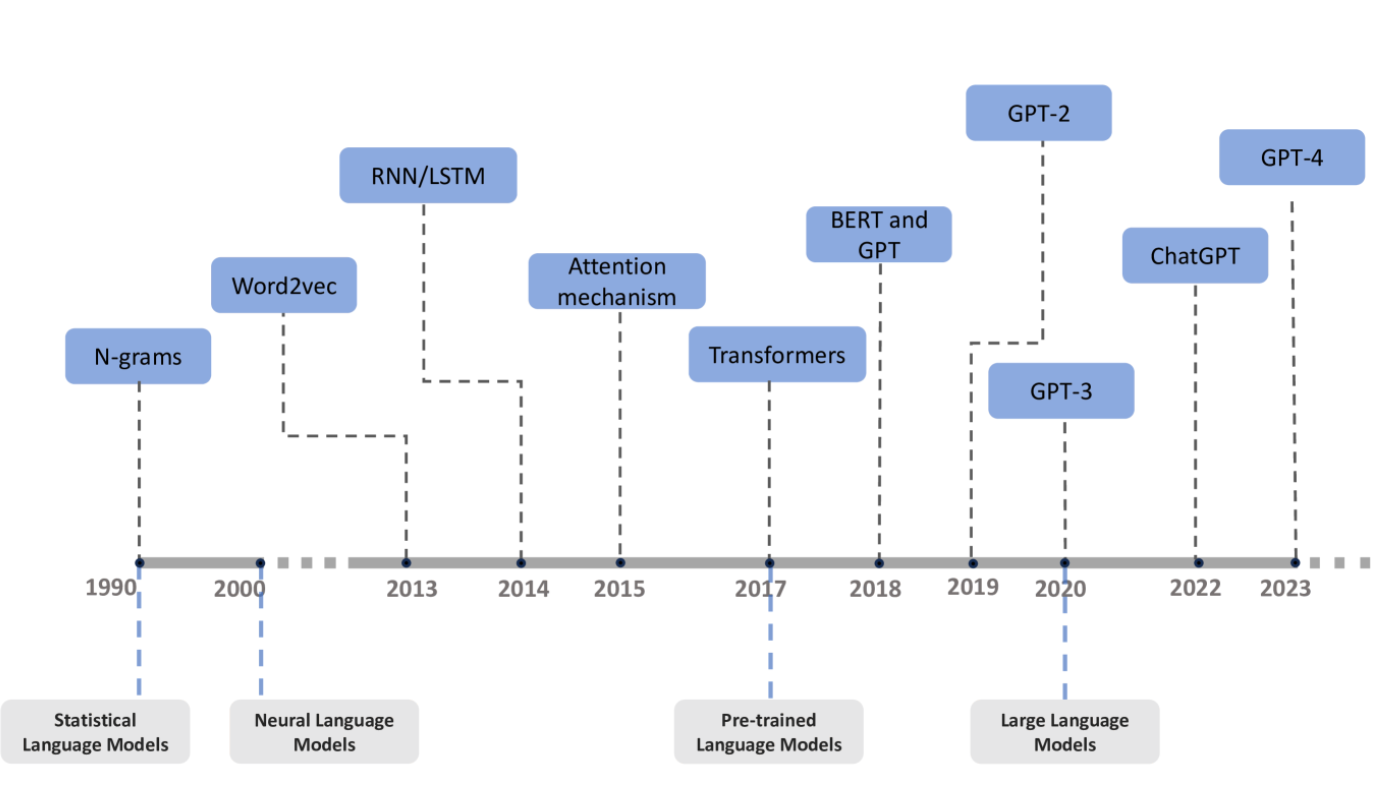
\includegraphics[width=0.8\linewidth]{img/chap04/historyllm.png}
    \caption{History and development of language models}
    \label{fig:historyllm}
\end{figure}

\section{Rule-based Language Model}

In the early days of NLP, rule-based language models were the dominant paradigm for enabling computers to process and generate human language. These models operated on the principle of explicitly programming a set of linguistic rules that dictated how language should be understood or produced. These rules were typically based on grammatical principles, syntactic structures, and semantic relationships that linguists and programmers manually codified.

The core mechanism of a rule-based language model involved defining a system of rules to analyze input text or to generate output text. For natural language understanding (NLU) tasks, these rules might involve pattern matching, keyword identification, and parsing techniques to extract meaning or identify the intent behind a user's input. For natural language generation (NLG) tasks, rules would specify the grammatical structure, word order, and vocabulary to construct coherent and syntactically correct sentences.

Consider a simplified example of a rule-based system for intent classification in a customer service context. Rules could be defined as follows:

\begin{itemize}
    \item If the input contains the keywords "\textit{cancel order}" or "\textit{return item}", classify the intent as "\textit{Order Modification}".
    \item If the input contains the keywords "\textit{track package}" or "\textit{check shipping status}", classify the intent as "\textit{Shipping Inquiry}".
    \item If the input contains the keywords "\textit{change password}" or "\textit{account login}", classify the intent as "\textit{Account Management}".
\end{itemize}

When a user enters a query, the system would scan the input for these predefined keywords and apply the corresponding rule to determine the user's intent.

Similarly, for a basic rule-based system for generating greetings, rules might be:

\begin{itemize}
    \item If the time of day is before 12:00 PM, output "\textit{Good morning}".
    \item If the time of day is between 12:00 PM and 5:00 PM, output "\textit{Good afternoon}".
    \item If the time of day is after 5:00 PM, output "\textit{Good evening}".
\end{itemize}

These examples illustrate the fundamental principle of rule-based models: direct, manual encoding of linguistic knowledge into a set of instructions.

However, these systems suffered from significant limitations. The complexity and variability of natural language made it incredibly difficult to create a comprehensive set of rules that could handle all possible linguistic phenomena. Natural language is full of nuances, exceptions, idiomatic expressions, and context-dependent meanings that are hard to anticipate and program explicitly. As a result, rule-based systems often proved to be brittle and unable to generalize to inputs that deviated even slightly from the predefined patterns. They required extensive manual effort to develop and maintain, and their performance plateaued relatively quickly as the complexity of the language tasks increased.

The foundation of large language models can be traced back to experiments with neural networks and neural information processing systems that were conducted in the 1950s to allow computers to process natural language. Researchers at IBM and Georgetown University worked together to create a system that would be able to automatically translate phrases from Russian to English. As a notable demonstration of machine translation, research in this field took off from there.

The idea of LLMs was first floated with the creation of Eliza in the 1960s: it was the world’s first chatbot, designed by MIT researcher Joseph Weizenbaum. Eliza marked the beginning of research into natural language processing (NLP), providing the foundation for future, more complex LLMs.

ELIZA relies on a pattern-matching algorithm, where the user’s input is parsed for key phrases, and corresponding predefined responses are generated. Its working can be broken down into the following steps:

\begin{itemize}
    \item Input Processing: ELIZA takes user input and searches for specific keywords or phrases.
    \item Pattern Matching: When a match is found, the program applies simple rules to generate a response. These rules are not based on deep understanding but on syntactic structures.
    \item Response Generation: The output is a reformulation of the input, often transformed into a question. If no keywords are detected, ELIZA resorts to generic responses such as “Tell me more” or “Why do you say that?”
\end{itemize}

An example of a conversation with ELIZA could go like this:

User: "I feel sad today."

ELIZA: "Why do you feel sad today?"

This simplistic method created the illusion of understanding and empathy, a hallmark of many early chatbots.

Weizenbaum was attempting to prove his assumption that the communications between humans and machines were fundamentally superficial, but things didn’t work out as planned. To simplify the experiment and minimize disputes, Weizenbaum developed a program using “active listening,” which did not require a database storing real-world information, but would reflect back a person’s statements to carry the conversation forward. 

He was surprised and horrified that people, including Weizenbaum’s own secretary, described the computer program as having human-like feelings. Weizenbaum wrote: “\textit{My secretary, who had watched me work on the program for many months and therefore surely knew it to be merely a computer program, started conversing with it. After only a few interactions with it, she asked me to leave the room}”. He later added, “\textit{I had not realized … that extremely short exposures to a relatively simple computer program could induce powerful delusional thinking in quite normal people}”.

ELIZA’s creation was a pivotal moment in the history of AI, particularly in natural language processing and human-computer interaction. It demonstrated that computers could engage in simulated conversations, paving the way for more complex conversational agents like modern chatbots and voice assistants (e.g., Siri, Alexa, ChatGPT).

Psychological Effects: ELIZA revealed that people were willing to project human-like qualities onto machines, an observation that later became known as the ELIZA effect. Despite the program’s simplistic mechanics, users often felt that ELIZA understood them, highlighting the potential for computers to evoke emotional responses from humans.

Inspiration for Modern Chatbots: ELIZA was the precursor to modern chatbots and virtual assistants that use advanced NLP techniques like deep learning, intent recognition, and context awareness to carry out much more sophisticated interactions.

Ethical Considerations: ELIZA also sparked early discussions about the ethical implications of AI in therapy and other human-centered fields. Weizenbaum himself became critical of using AI in roles that require genuine understanding, like psychotherapy, fearing that people might overestimate the capabilities of such systems.

\section{Statistical Language Models (SLMs)}

The advent of statistical language models (SLMs) in the late 20th century marked a crucial turning point, as these models began to learn language patterns directly from large amounts of data, offering a more flexible and scalable approach that eventually superseded rule-based methods for most NLP applications. Rule-based systems, while historically significant as an initial step in computational language processing, are rarely used as the primary approach today, except in very narrow and well-defined domains where the linguistic scope is highly restricted.

Statistical Language Models, or Count-based models, originated in the 1990s as mathematical models addressing contextually relevant properties of natural language from a probabilistic statistical perspective. 

The essence of statistical language modeling lies in ascertaining the probability of a sentence occurring within a text. Considering $S$ as the sentence "\textit{I am very happy}", $P(w_i)$ signifies the probability of the $i$-th word in the sentence: $w_1$ as "I", $w_2$ as "am", $w_3$ as "very", and $w_4$ as "happy". Now, the objective is to ascertain the likelihood of $S$ appearing in the text, denoted as $P(S)$:

\begin{equation}
P(S) = P(w_1, w_2, w_3, w_4) = P(I, am, very, happy)
\end{equation}

\noindent To calculate this probability, the conditional probability can be employed:

\begin{equation}
P(I, am, very, happy) = P(I) \cdot P(am \mid I) \cdot P(very \mid I, am) \cdot P(happy \mid I, am, very)
\end{equation}

\noindent where $P(I)$ represents the probability of the word ``I" appearing and $P(am \mid I)$ stands for the probability of ``am" appearing given that ``I" has appeared. When we multiply $P(am \mid I)$ by $P(I)$, it fulfills the condition of "I" appearing in $P(am \mid I)$, resulting in the probability of ``I am" appearing together as $P(I, am) = P(I) \cdot P(am \mid I)$. 

\noindent In general, the probability of a sequence of $K$ words is calculated using the chain rule as:

\begin{equation}
P(w_1 w_2 \ldots w_K) = P(w_1) P(w_2 | w_1) \cdots P(w_K | w_1 w_2 \ldots w_{K-1}) = \prod_{k=1}^{K} P(w_k | w_1 w_2 \ldots w_{k-1})
\end{equation}

Now, the question arises: how do we calculate the conditional probability of the occurrence of each word? The answer lies in Maximum Likelihood Estimation, enabling us to estimate probabilities by substituting them with frequencies when the sample size is sufficiently large, given by:

\begin{equation}
P(w_k \mid w_1 w_2 \cdots w_{k-1}) = \frac{P(w_1 \cdots w_{k-1} w_k)}{P(w_1 w_2 \cdots w_{k-1})} = \frac{C(w_1 w_2 \cdots w_k)}{C(w_1 w_2 \cdots w_{k-1})}
\end{equation}

\noindent where $C(\cdot)$ represents the count of occurrences of the subsequence in the training set. Using this formula, we can calculate the likelihood of each word as the $i$-th word given the preceding $k - 1$ words. Then, we select the $k$-th word by choosing the word associated with the highest probability. 

However, the larger $K$ is, the lower the frequency of occurrence of a $K$-word sequence, and there will be cases where the frequency of occurrence of the previous $K - 1$ words is high, causing the probability $P(w_k | w_1 w_2 \ldots w_{k-1})$ to be nearly zero. This leads to the $K$-word sequence almost never occurring (simply put, the sequence does not appear in the training data).\\

\subsection{N-gram Language Model}

To reduce this problem, instead of using $K - 1$ previous words, we only use $N - 1$ previous words (assumes that the $N$-th word is related to the initial $N - 1$ words). This leads us to the concept of \textbf{N-gram Language Models}:

\begin{equation}
    P(w_k | w_1 w_2 \ldots w_{k-1}) = P(w_k | w_{k-N+1} w_{k-N+2} \ldots w_{k-1})
\end{equation}

The probability of a sequence of words is calculated as:

\begin{equation}
    P_N(W) = \prod_{k=1}^{K} P(w_k | w_{k-N+1} w_{k-N+2} \ldots w_{k-1})
\end{equation}

Typically, $N$ is chosen as 1, 2, or 3.\\

This model is also known as a \textbf{(N-1)-order Markov Model}.\\

However, this model has the following drawbacks:

\begin{itemize}
    \item \textbf{Violation of dependency condition}: The transition from $K - 1$ to $N - 1$ is not theoretically valid from the start.
    \item \textbf{Saturation}: With enough data, the model performs better, but at some point, adding more data does not change the probability distribution. This happens especially with bigrams and trigrams, where the number of combinations can reach billions.
    \item \textbf{Lack of generalization}: Different topics, styles, and structures have different word combinations. Thus, with different data sources, model quality varies greatly—especially when training on one type of writing but testing on another. This leads to poor generalization and performance.
\end{itemize}

N-gram model also efficiently computes conditional probabilities. It is necessary to pre-compute and save $C(X)$ required for the conditional probability computation, where $X$ is a sentence of length $n$. The number of possible sentences $X$ grows exponentially with the size of the vocabulary. For instance, with 1000 different words, there exist $1000^n$ potential sequences of length $n$. However, excessively large values of $n$ pose storage limitations. Typically, $n$ is confined to 2 or 3, causing each word to relate to only its first 1 or 2 preceding words, ultimately leading to a reduction in the model’s accuracy.

\subsection{Structured Language Models}

Statistical Language Models have long been central to natural language processing tasks, from speech recognition to machine translation. Traditional SLMs, particularly n-gram models, estimate the probability of a word based on a fixed number of preceding words. Take the previous case as an example, a trigram model might estimate the probability of the word “happy” based on the two previous words of the sentence S: $\mathbf{P}(\text{happy} | \text{am},\text{very})$

While effective for short contexts, n-gram models suffer from significant limitations: they use fixed-length context windows, ignore grammatical structure, and perform poorly when encountering rare or unseen word combinations.

To overcome these challenges, Structured Language Models were introduced. These models extend statistical approaches by incorporating syntactic structures, such as parse trees, into the language modeling process. Rather than treating text as a flat sequence of words, Structured LMs incrementally build syntactic structures as sentences unfold, jointly modeling the likelihood of words and their grammatical relationships.

For example, in the sentence: \textit{The keys to the cabinet are missing}, a traditional trigram model might incorrectly favor “is” over “are” due to its short context. However, a structured LM can parse that “keys” is the true subject of the sentence and correctly predict the plural verb “are” by capturing the syntactic relationship between the subject and verb, regardless of intervening nouns like “cabinet”.

\begin{forest}
  for tree={align=center, parent anchor=south, child anchor=north, l sep=15pt}
  [S
    [$\text{NP}_{pl}$
      [DT [The]]
      [NNS [keys]]
      [PP
        [P [to]]
        [NP
          [DT [the]]
          [NN [cabinet]]
        ]
      ]
    ]
    [$\text{VP}_{pl}$
      [VBP [are]]
      [ADJP
        [VBG [missing]]
      ]
    ]
  ]
\end{forest}

Syntax tree of the sentence "The keys to the cabinet are missing".

Structured LMs offer several key improvements over generic SLMs:

\begin{itemize}
    \item Long-Range Dependency Modeling: Structured LMs are not limited by fixed context windows. They can use hierarchical parse trees to capture dependencies between distant words, improving grammatical coherence.
    \item Better Generalization: By leveraging syntactic roles (e.g., subject, verb, object), Structured LMs generalize better to unseen sequences. Even if a specific phrase hasn’t been encountered during training, its structure may match other known patterns.
    \item Reduced Data Sparsity: Instead of learning from exact word sequences, Structured LMs abstract over syntactic categories. This reduces the zero-probability problem common in high-order n-gram models.
    \item Joint Prediction: Structured LMs jointly predict words, parts-of-speech, and parse decisions, creating a richer and more integrated model of language generation.
\end{itemize}

A well-known example of Structured LM is the model developed by Chelba and Jelinek (2000), which incrementally constructs a binary parse tree while predicting each word in a sentence. This model demonstrated lower perplexity and improved accuracy in speech recognition tasks compared to traditional n-gram baselines.

\section{Neural Language Models (NLMs)}

Neural Language Models leverage neural networks to predict the probabilities of subsequent words within sequences. They effectively handle longer sequences and mitigate the limitations associated with small $n$ in SLMs. 

NLMs operate akin to the n-gram concept, assuming that the probability of each word depends only on its previous $n-1$ words. The first layer—the input layer—concatenates the word vectors of $n-1$ words, forming a vector $X \in \mathbb{R}^{m \times (n-1)}$. Subsequently, the second layer—the hidden layer—derives the output $H$ by applying a non-linear activation function, like sigmoid or tanh, to the matrix product of $X$ and $W_{xh}$. Following this, the third layer—the output layer—aims to forecast the subsequent word based on the hidden layer’s output. With $|V|$ neurons within the output layer, the resulting output vector $O \in \mathbb{R}^{|V|}$ is computed by multiplying $H$ and $W_{ho}$. This resultant vector then undergoes the Softmax function, producing a vector $O'$ containing the probability value assigned to each word.

The Softmax function, concerning the output of the $i$-th neuron, is defined as follows:

\begin{equation}
    O'_i = \text{Softmax}(O'_i) = \frac{\exp(O_i)}{\sum_{j=1}^{|V|} \exp(O_j)}
\end{equation}

\noindent where $O'_i$ denotes the output value of the $i$-th node, and $|V|$ represents the count of output nodes, corresponding to the classification categories. Utilizing the Softmax function allows the transformation of output values from multiclassification into a probability distribution, ensuring a sum of 1 within the range $[0, 1]$.

\begin{figure}[h]
    \centering
    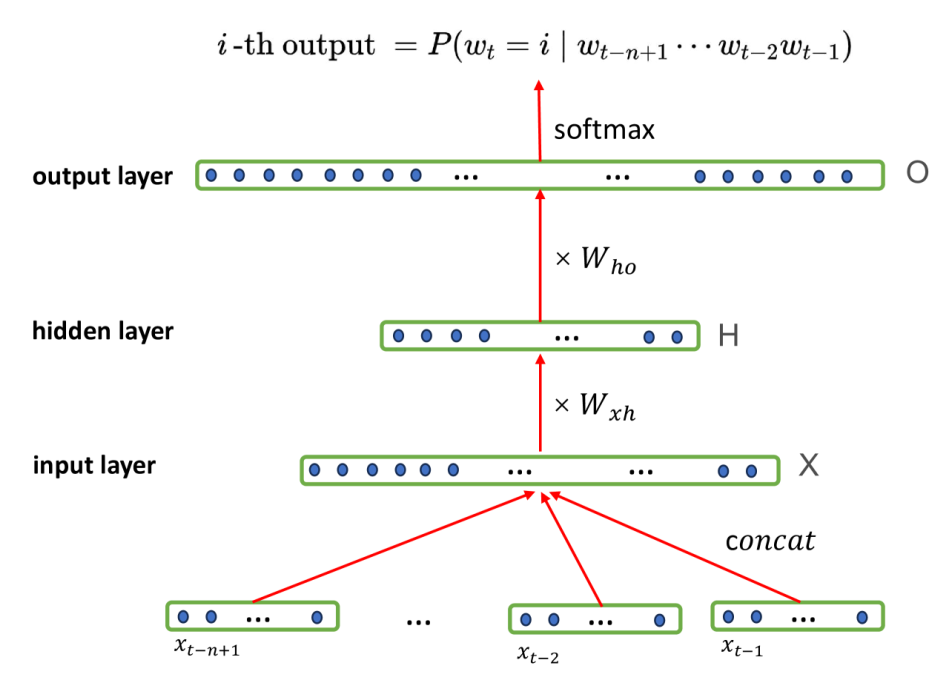
\includegraphics[width=0.8\linewidth]{img/chap04/neuralmodel.png}
    \caption{A Neural Language Model}
    \label{fig:neuralmodel}
\end{figure}

Neural Language Models can solve data sparseness of N-gram Language Models. It can be further classified into Feed Forward Neural Networks (FNNs) and Recurrent Neural Networks (RNNs).

Every NLM has the same kind of input and output:

\begin{itemize}
    \item Input: Word embedding or character embedding (strings and characters to real vectors in an $n-$dimensional space.
    \item Output: For each output unit, it represents the probability of a word or character given the context. What "context" means depends on the type of model being used. For Feedforward Neural Networks (FNNs), the context is a fixed-length sequence consisting of the words or characters immediately preceding the current character being considered. This is similar to N-gram Language Models. For Recurrent Neural Networks (RNNs), the context is like that of FNNs but with variable length. This type helps address the limited context problem of FNNs—meaning it is no longer restricted to N-grams, and the shortcomings of N-gram Language Models are resolved.
\end{itemize}

\textbf{Neural Probabilistic Language Model}

The \textbf{Neural Probabilistic Language Model (NPLM)}, proposed by \textbf{Yoshua Bengio et al. in 2003}, was a landmark in the history of natural language processing (NLP) and deep learning. It was the first major \textit{neural language model}, designed to overcome the limitations of statistical n-gram models, such as:

\begin{itemize}
    \item \textbf{Data sparsity}
    \item \textbf{Poor generalization to unseen sequences}
    \item \textbf{Fixed-size context windows}
\end{itemize}

The NPLM introduced two core innovations:

\begin{enumerate}
    \item \textbf{Word embeddings}: Learn dense vector representations of words.
    \item \textbf{Feedforward neural network}: Predict the next word using the learned embeddings.
\end{enumerate}

\textbf{Model Architecture}

\begin{itemize}
    \item \textbf{Input:} A context of $n-1$ words $(w_1, w_2, \ldots, w_{n-1})$.
    \item \textbf{Embedding Layer:} Each word $w_i$ is mapped to a vector $C(w_i) \in \mathbb{R}^d$. These are concatenated into $x \in \mathbb{R}^{(n-1) \cdot d}$.
    \item \textbf{Hidden Layer:}
    \[
        h = \tanh(Wx + b)
    \]
    where $W$ is the weight matrix, $b$ is a bias vector.
    \item \textbf{Output Layer:}
    \[
        y = b' + Uh
    \]
    where $U$ is the output weight matrix and $b'$ is the bias vector.
    \item \textbf{Softmax Layer:}
    \[
        P(w_t = i \mid w_{t-n+1}, \ldots, w_{t-1}) = \frac{\exp(y_i)}{\sum_{j=1}^{|V|} \exp(y_j)}
    \]
\end{itemize}

\textbf{Key Contributions}

\begin{itemize}
    \item \textbf{Word embeddings}: Represent words in a continuous vector space capturing semantic similarity.
    \item \textbf{Parameter sharing}: Same parameters are used across all word positions, leading to better generalization.
    \item \textbf{Joint learning}: The model learns both word representations and a language model.
\end{itemize}

\textbf{Limitations at the Time}

\begin{itemize}
    \item Computationally expensive due to large vocabulary softmax.
    \item Fixed-size context window; could not model long-range dependencies.
\end{itemize}

These limitations were later addressed by models such as:

\begin{itemize}
    \item \textbf{Word2Vec (2013)}: Efficient embedding training.
    \item \textbf{RNNs, LSTMs}: Sequence modeling with variable context.
    \item \textbf{Transformers}: Parallelized long-range dependency modeling.
\end{itemize}

Reference

Bengio, Y., Ducharme, R., Vincent, P., \& Jauvin, C. (2003). \textit{A Neural Probabilistic Language Model}. Journal of Machine Learning Research, 3(Feb), 1137–1155. \\
\url{https://www.jmlr.org/papers/volume3/bengio03a/bengio03a.pdf}

\textbf{The concept of word vectors}

Humans effortlessly comprehend word meanings. For instance, “cat” and “dog” share closer semantic connections than “cat” and “tree” since they both represent animals. But how does a computer accomplish this? Computers operate using binary code — 0s and 1s — so human language needs translation into binary. Word vectors can accomplish this, which are numerical representations of human language, where each word corresponds to a distinct vector. These vectors usually possess fixed dimensions and can simulate word relationships through the angles between them. An intriguing example is the angle between the word vectors for “cat” and “dog” which is smaller than the angle between the word vector for “cat” and “tree”. Word2Vec is a widely recognized tool for computing word vectors. Its function involves converting words into dense numerical representations, making words with similar semantics closer together in the vector space.

The efficacy of Word2Vec is notably influenced by its utilization of neural networks, which mirrors the structure and functionality of the human brain, comprising interconnected simple units known as neurons organized into different layers. Figure~2 provides a visualization of a simple NLM structure, composed of input, hidden, and output layers. Within this structure, each word vector $x_t \in \mathbb{R}^m$, the matrix $W_{xh} \in \mathbb{R}^{m(n-1) \times h}$, and the matrix $W_{ho} \in \mathbb{R}^{h \times |V|}$, where $h$ signifies the number of neurons in the hidden layer, and $V$ is the vocabulary containing all words recognized by the model.

Word2Vec focuses solely on learning word embeddings rather than modeling full word distributions. This design decision simplifies the model and allows it to scale efficiently.

\textbf{Model Simplification}

Word2Vec uses a shallow neural network with only input and output layers, eliminating hidden layers entirely. It offers two architectures:
\begin{itemize}
    \item \textbf{CBOW (Continuous Bag-of-Words)}: Predicts a word given its context.
    \item \textbf{Skip-Gram}: Predicts context words given a target word.
\end{itemize}

\textbf{Efficient Training with Approximate Objectives}

Instead of using full softmax, Word2Vec employs:

\begin{itemize}
    \item \textbf{Negative Sampling}: Samples a small number of ``negative'' examples for contrastive learning.
    \item \textbf{Hierarchical Softmax}: Uses a binary tree to reduce softmax complexity from $O(|V|)$ to $O(\log |V|)$.
\end{itemize}

These methods drastically reduce training time and memory usage, making it possible to train on corpora with billions of words.

\textbf{Scalability and Practicality}

Due to its lightweight architecture and efficient training, Word2Vec can be applied to very large datasets and has been successfully used to train embeddings on datasets like Google News, Wikipedia, and Common Crawl.

\subsection{Recurrent Neural Network \& Long-Short Term Memory}

Recurrent Neural Networks stand as a cornerstone in the development of artificial intelligence, particularly in the processing of sequential data. Distinct from traditional neural networks, RNNs have the unique ability to retain information from previous inputs, thanks to their internal memory mechanism. This feature makes them exceptionally suitable for tasks where the context and order of data are pivotal, such as in language processing, time series analysis, and speech recognition.

The core functionality of RNNs lies in their looped architecture, which allows information to persist. In an RNN, each unit passes its output back as an input to itself in the subsequent step, creating a form of internal memory. This looping mechanism enables the network to remember past information and use it to influence future outputs. However, this memory is inherently short-lived, a characteristic that serves both as an advantage and a limitation.

RNNs have been effectively employed in a variety of applications where sequential data plays a critical role. In the realm of language modeling and text generation, they can predict the next word in a sentence based on the preceding words. In the field of speech recognition, RNNs are instrumental in understanding the temporal dynamics of spoken language. Additionally, their ability to process time-series data makes them invaluable in areas like stock market prediction and weather forecasting.

Despite their versatility, RNNs face significant limitations, particularly the issue of vanishing gradients. This problem arises when the network struggles to learn and retain information from long sequences, as the gradient—essential for the network's learning process—tends to either vanish or explode during back-propagation through time and layers. This makes it challenging for RNNs to learn long-range dependencies within data sequences.

To address these limitations, a new architecture known as Long Short-Term Memory (LSTM) was developed. LSTMs, while being a type of RNN, include a crucial modification: the incorporation of gates (input, forget, and output gates) that regulate the flow of information. These gates efficiently determine which information should be retained or discarded, enabling LSTMs to maintain longer memory. Consequently, LSTMs can effectively learn from extended sequences of data, significantly enhancing the performance of neural networks in tasks requiring the understanding of long-range dependencies.

Long Short-Term Memory (LSTM) networks have been a significant breakthrough in the field of artificial intelligence, particularly in handling sequences of data. Originating as an advanced form of Recurrent Neural Networks (RNNs), LSTMs were designed to overcome the challenges of learning long-range dependencies, a limitation inherent in traditional RNNs. The key innovation in LSTMs is their use of a gated mechanism, consisting of input, forget, and output gates, which regulates the flow of information. This design allows LSTMs to retain information over longer periods, making them highly effective for complex tasks in natural language processing, speech recognition, and time-series analysis.

While LSTMs represent a significant advancement over traditional RNNs, they are not without their own limitations. One major issue is their computational complexity and inefficiency, primarily due to the sequential nature of their processing. LSTMs struggle with processing very long sequences, as the time and computational resources required scale linearly with the sequence length. Additionally, LSTMs still face challenges with vanishing gradients, albeit to a lesser extent than RNNs, especially in very deep networks or extremely long sequences. This makes them less practical for some real-world applications that involve massive datasets or require rapid processing.

\subsection{Transformers \& Pre-trained Language Models (PLMs)}

The landscape of Natural Language Processing (NLP) underwent a monumental shift with the introduction of the Transformer architecture. This innovative neural network design, detailed in the seminal paper "Attention is All You Need", creatively synthesized ideas from predecessor architectures to overcome their inherent limitations, particularly in handling long-range dependencies in text. The advent of Transformers was not merely an incremental improvement; it laid the foundation for the development of Pre-trained Language Models (PLMs), which have revolutionized how machines understand and generate human language.

Prior to Transformers, Recurrent Neural Networks (RNNs), especially their advanced form, Long Short-Term Memory (LSTM) networks, were the dominant architectures for processing sequential data like text. As we discussed previously, LSTMs addressed the vanishing gradient problem of traditional RNNs through a gated mechanism, enabling them to learn long-range dependencies to some extent. However, LSTMs processed sequences sequentially, which limited their parallelization capabilities and made them computationally expensive for very long sequences.

The Transformer architecture introduced a paradigm shift by primarily relying on the self-attention mechanism. Unlike the sequential processing of RNNs, self-attention allows the model to simultaneously weigh the importance of different words in a sequence when processing a particular word. This mechanism enables the model to directly capture both short and long-range relationships between words, regardless of their distance in the input sequence. The sources highlight that the Transformer model consists of multiple layers of self-attention and feedforward neural networks, which work in concert to learn contextual representations of words and their intricate relationships within a text. This architecture demonstrated superior performance in various NLP tasks and quickly became the backbone of state-of-the-art language models.

\textbf{Understanding Transformer Models: Self-Attention Mechanism}

At the heart of the Transformer model is the self-attention mechanism. This allows the model to process different parts of the input sequence in parallel, as opposed to the sequential processing in RNNs and LSTMs. Self-attention enables the model to weigh the importance of different words in a sentence, regardless of their positional distance from each other. For example, in the sentence "The cat, which was hungry, meowed loudly," the model can directly relate "cat" to "meowed" for better context understanding, something that is more challenging in traditional sequential models.

Architecture Details:

\begin{itemize}
    \item Encoder and Decoder Stacks: The Transformer model consists of an encoder to process the input and a decoder to produce the output. Both the encoder and the decoder are composed of a stack of identical layers, typically six in number.
    \item Encoder: Each encoder layer has two sub-layers. The first is the multi-head self-attention mechanism, and the second is a simple, position-wise fully connected feed-forward network.
    \item Decoder: Each layer in the decoder also has two sub-layers (like the encoder) but adds a third one, which performs multi-head attention over the output of the encoder stack.
    \item Positional Encoding: Since Transformers do not use recurrence, they incorporate positional encodings to give the model information about the relative or absolute position of the words in the sequence. This encoding is added to the input embeddings at the bottoms of the encoder and decoder stacks.
\end{itemize}

\begin{figure}[h]
    \centering
    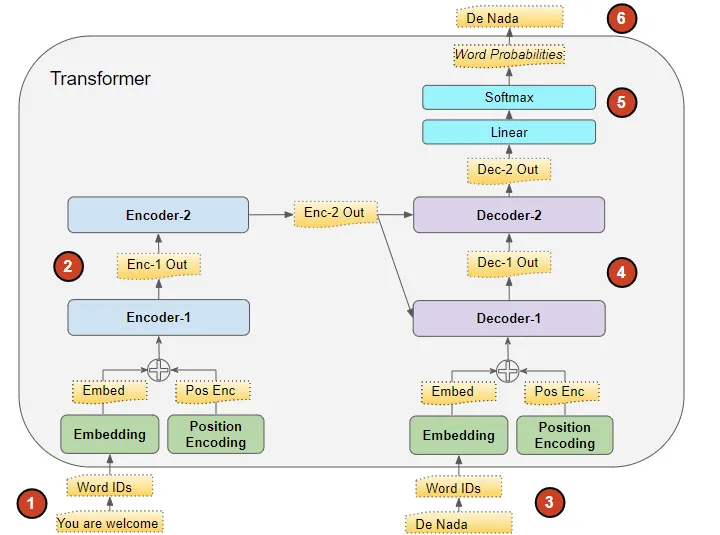
\includegraphics[width=0.8\linewidth]{img/chap04/transformer-arch.png}
    \caption{Architecture of a Transformer}
    \label{fig:transformer-arch}
\end{figure}

Advantages of Transformers:

\begin{itemize}
    \item Parallelization: Unlike RNNs and LSTMs, Transformers process data in parallel, significantly speeding up training.
    \item Handling Long-range Dependencies: Thanks to the self-attention mechanism, Transformers can manage long-range dependencies in text better than RNNs and LSTMs.
    \item Flexibility and Scalability: The architecture is highly flexible and scalable, making it effective for a wide range of tasks beyond NLP, such as image recognition and generation.
\end{itemize}

In this picture is the development by year and the classification of Transformer models:

\begin{figure}[h]
    \centering
    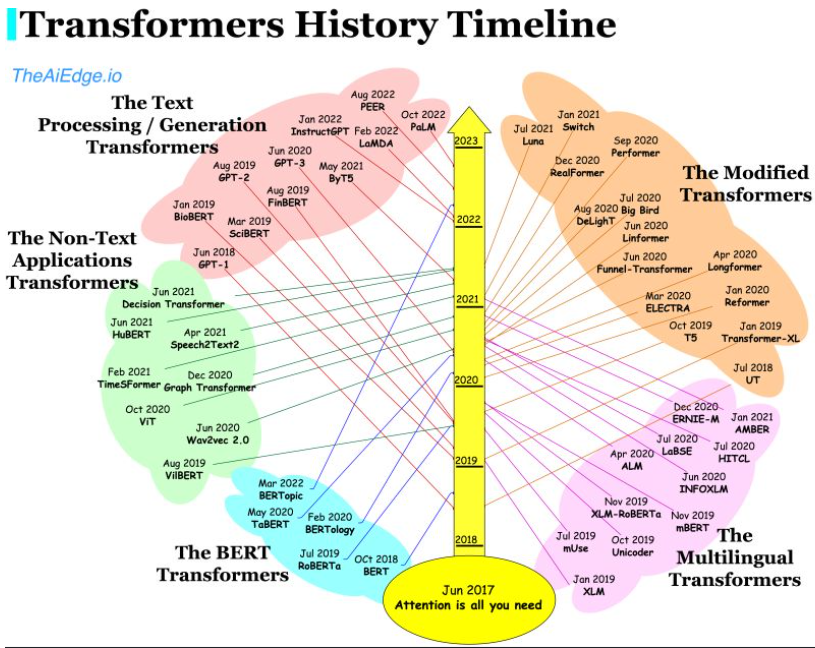
\includegraphics[width=0.8\linewidth]{img/chap04/transformer-history.png}
    \caption{History of Transformers}
    \label{fig:transhist}
\end{figure}

Transformer models have diversified into several distinct classes, each tailored to specific applications and challenges in the field of artificial intelligence.

Processing/Generation Transformers are designed for either interpreting existing text or generating new content. Processing models excel in tasks like sentiment analysis and text classification, adeptly analyzing and extracting insights from language. On the other hand, Generation models are employed for creative tasks like storytelling or text generation, where they generate coherent and contextually relevant text.

In the realm of \textit{Modified Transformers}, various adaptations of the original Transformer architecture aim to enhance performance or efficiency. These models include architectures like the Reformer, which reduces memory consumption, or those with altered attention mechanisms for specific data types or tasks, addressing challenges like handling longer sequences or improving computational efficiency.

\textit{Non-Text Transformers} represent a significant expansion of the Transformer's application, extending beyond traditional natural language processing. These models process data like audio, genomic sequences, or images, leveraging the Transformer architecture to capture complex relationships in non-textual domains. For instance, the Vision Transformer (ViT) adapts the Transformer approach to image processing tasks.

\textit{BERT Transformers}, inspired by Google's BERT, focus on understanding and analyzing language. This class includes models like RoBERTa, DistilBERT, and ALBERT, each building upon or refining the approach of BERT. These models are particularly effective in tasks like text classification, question answering, and language inference, offering deep contextual insights into language.

\textit{Multimodal Transformers} represent a groundbreaking class that processes and generates multiple types of data, such as text and images. Models like OpenAI’s DALL-E and CLIP are prime examples, capable of generating images from text descriptions or understanding concepts across both visual and textual modalities. These models are pioneering in AI, enabling applications like image captioning, visual question answering, and cross-modal translation.

The effectiveness of the Transformer architecture paved the way for the rise of Pre-trained Language Models (PLMs). The principle behind PLMs is to first train a large-scale model on an extensive volume of unlabeled text data to grasp fundamental language structures, including vocabulary, syntax, semantics, and logic – a phase known as pre-training. This pre-training process allows the model to learn general linguistic knowledge from vast amounts of text.

Several training techniques are employed during pre-training. One prominent technique is Masked Language Modeling (MLM), where a certain proportion of tokens in the input sequence are masked, and the model is trained to predict the masked tokens based on the surrounding context. The source indicates that MLM encourages the model to learn meaningful representations of language that can generalize to a wide range of downstream tasks. Another fundamental pre-training objective is Language Modeling (or next token prediction), where the model learns to predict the next word in a sequence given the preceding words.

Once the pre-trained model has acquired a broad understanding of language, it can be adapted to perform specific NLP tasks like text classification, question answering, and text summarization through a process called fine-tuning. Fine-tuning involves further training the pre-trained model on a smaller, task-specific dataset. This "pre-training and fine-tuning" paradigm has proven highly effective, as the pre-trained model's general language knowledge provides a strong foundation for learning task-specific patterns, often requiring significantly less task-specific data and computational resources compared to training models from scratch.

Numerous influential PLMs have emerged based on the Transformer architecture. Models like BERT, which primarily utilizes the MLM objective, excel at tasks requiring a deep understanding of context. The GPT series (including GPT-2, GPT-3, and GPT-4), which employs the next token prediction objective, has demonstrated remarkable capabilities in text generation. Other notable PLMs mentioned in the sources include RoBERTa, PaLM, and LLaMA. These models, trained on massive datasets containing billions of words, have pushed the boundaries of what NLP models can achieve.

The sources highlight several benefits of using PLMs. Their ability to capture general linguistic knowledge allows them to achieve strong performance on a wide range of downstream tasks. The transfer learning capability significantly reduces the need for large amounts of labeled data for each specific task, making NLP more accessible and efficient. Furthermore, the pre-trained weights provide a strong initialization, leading to faster convergence and improved performance during fine-tuning.

To further enhance the efficiency of adapting PLMs, parameter-efficient fine-tuning (PEFT) techniques have been developed. These methods aim to adapt LLMs to specific datasets or domains by updating only a small subset of the model's parameters. Techniques like Adapters, which insert additional learnable layers into the Transformer architecture, and BitFit, which only updates the model's bias terms, allow for efficient fine-tuning while keeping the majority of the pre-trained weights frozen. This approach reduces the computational overhead and memory requirements associated with fine-tuning large models.

The evolution of language models continued with the emergence of Transformer architectures, which have largely surpassed RNNs and LSTMs due to their superior performance on large-scale datasets and their ability to handle long-range dependencies more effectively through the self-attention mechanism. Transformers can selectively attend to key pieces of information in text, allowing for parallel processing and overcoming the sequential processing limitations of RNNs.

Pre-trained Language Models undergo initial training using an extensive volume of unlabeled text, enabling them to grasp fundamental language structures such as vocabulary, syntax, semantics, and logic — a phase termed pre-training. Subsequently, this comprehensive language model can be applied to various NLP tasks like machine translation, text summarization, and questionanswering systems. To optimize its performance, models need to be trained a second time on a smaller dataset customized for a specific downstream task — a phase known as fine-tuning. martial arts principles. A large number of studies on PLMs have been built on this paradigm, which introduces different architectures e.g. GPT-2 and BERT.

\subsection{Large Language Models (LLMs)}

\begin{figure}[h]
    \centering
    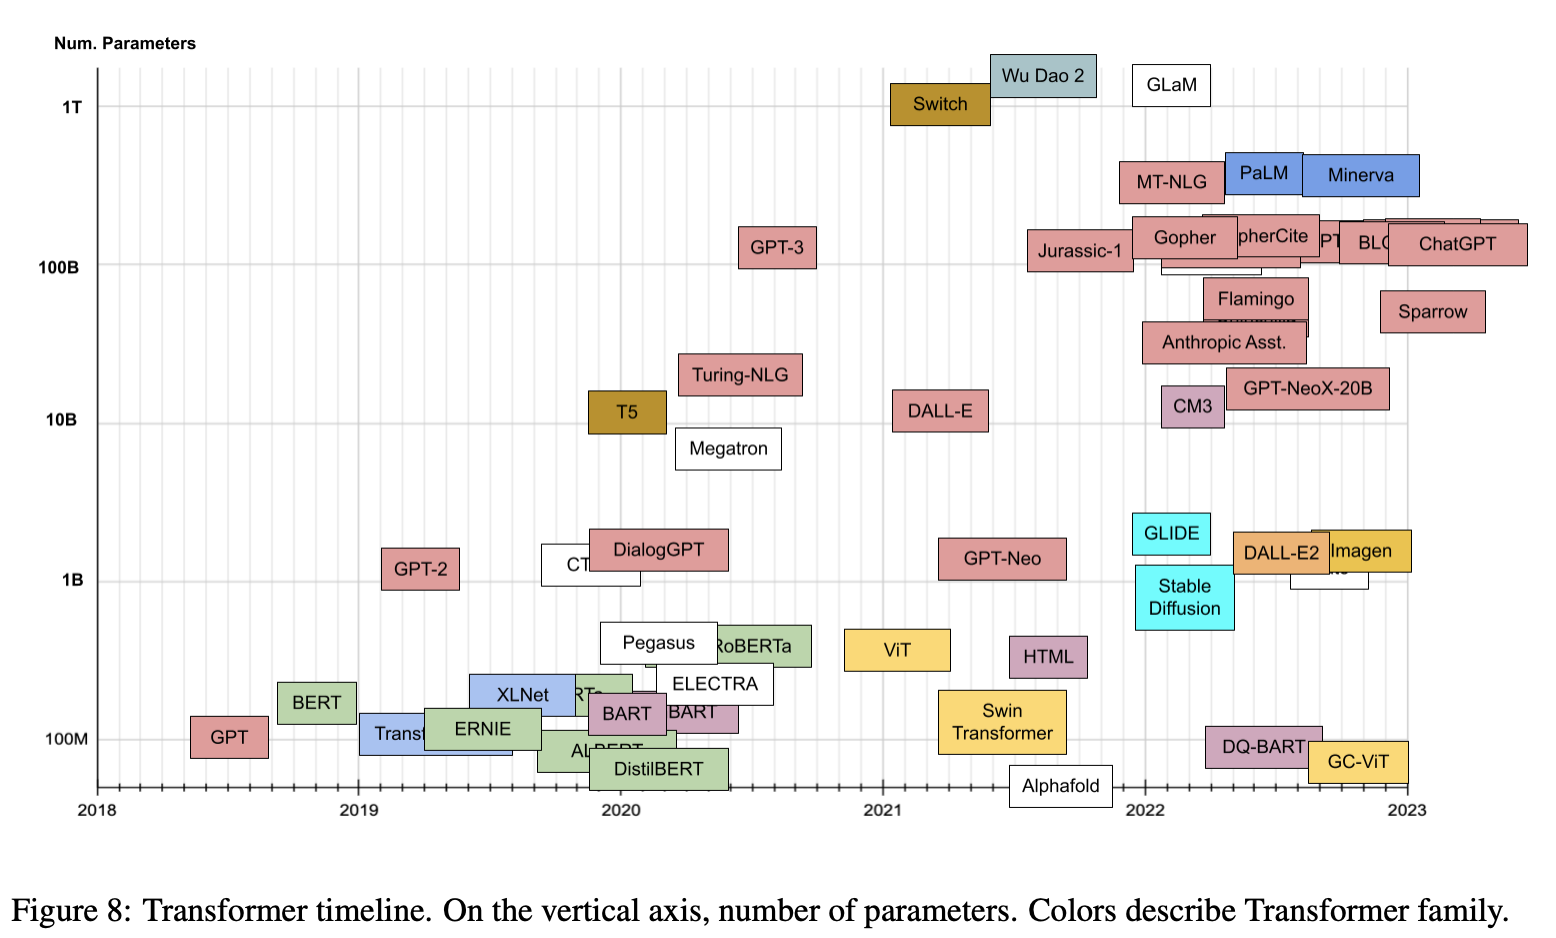
\includegraphics[width=0.8\linewidth]{img/chap04/numparam-transformer.png}
    \caption{Number of parameters of popular Neural Language Models}
    \label{fig:numparam-trans}
\end{figure}

LLMs are trained on massive text corpora with tens of billions (or more) of parameters, such as GPT-3 (Brown et al., 2020), GPT-4 (OpenAI, 2023), PaLM (Chowdhery et al., 2022), and LLaMA (Touvron et al., 2023). The goal of LLMs is to enable machines to understand human commands and adherence to human values. Their hallmark lies in the consolidation of two stages: initial pre-training on a vast general-purpose corpus followed by alignment with human values, rather than transitioning to a different domain. LLMs exhibit remarkable adaptability compared to PLMs, transitioning from specialized to general-purpose models. The substantial increase in model size, dataset volume, and computational prowess has resulted insignificant enhancements across various tasks and unveiled remarkable capabilities absent in smaller models. For example, GPT-3 has the capability to leverage contextual information, a functionality that GPT-2 (Radford et al., 2019) lacks. This means that when GPT-3 is prompted with task-related examples, it utilizes them to enhance its problem-solving capabilities. The number of parameters for LLMs typically exceeds a hundred billion, and the training data is usually in the range of a few hundred GB to a few TB. A concrete example is that there are multiple versions of the GPT-2 model, with the largest version having 1.5 billion parameters and using 40GB of text data for training. In contrast, the largest version of the GPT-3 model has 175 billion parameters and uses 570GB of text data for training. This example illustrates the significant discrepancy between LLMs and PLMs concerning parameter count and training data volume.

The field of Natural Language Processing (NLP) has witnessed a remarkable evolution, culminating in the emergence of Large Language Models (LLMs). These sophisticated AI systems represent a significant leap forward in the ability of machines to understand, generate, and interact with human language. Building upon decades of research in language modeling, LLMs have captured widespread attention due to their impressive capabilities across a diverse range of tasks. To comprehend their impact, it is crucial to define what constitutes an LLM and to identify prominent examples based on the available sources.

Large Language Models (LLMs) can be understood as an extension of PLMs, characterized primarily by their massive scale in terms of number of parameters (often tens of billions or more) and the extensive datasets they are trained on. This increase in scale, coupled with advancements in computational power and algorithmic innovations, has led to emergent abilities and significantly enhanced performance compared to their predecessors. The goal of LLMs is to understand human commands and align with human values. They often exhibit remarkable adaptability, transitioning from specialized to general-purpose models.

The architecture that underpins many state-of-the-art LLMs is the Transformer. As discussed in the previous section, the Transformer architecture, with its reliance on the self-attention mechanism, allows the model to efficiently capture both short and long-range dependencies in text, overcoming the limitations of earlier sequential models like RNNs and LSTMs. The ability to process information in parallel and to weigh the importance of different words in a sequence has been crucial in enabling LLMs to handle vast amounts of data and learn complex linguistic structures.

The sources provide numerous examples of LLMs that exemplify these characteristics:

\begin{itemize}
    \item The GPT series of models (GPT-3, GPT-4) from OpenAI are frequently cited as prominent examples of LLMs. These models, trained on massive textual data, have demonstrated the ability to generate human-level text and perform language-based tasks with exceptional precision. GPT-4, in particular, has shown strong performance in professional exams and explaining legal concepts.
    \item PaLM (Pathways Language Model) is another LLM highlighted in the sources. It has been noted for its performance and is used in the Bard chatbot service.
    \item LLaMA (Large Language Model Meta AI) is mentioned as an open-source LLM trained on publicly accessible datasets. Smaller versions of LLaMA have been fine-tuned for specific tasks like medical question answering (ChatDoctor). Recently, LLaMA 2 has also been released.
    \item BloombergGPT is presented as a specialized LLM with 50 billion parameters, designed to excel in financial tasks while maintaining strong general language model performance.
    \item Other LLMs mentioned include LaMDA, a family of chatbot LLMs from Google, and open-access multilingual models like BLOOM.
\end{itemize}

The capabilities of LLMs are wide-ranging, spanning areas such as customer support through automated responses, content creation for articles and creative writing, computer programming through code generation, and research assistance by rapidly retrieving and summarizing information. They are being applied in specialized domains like medicine for medical question answering and information extraction, and law for legal question answering and text generation.

Despite their impressive advancements, the sources also highlight several limitations of LLMs. These include the issue of hallucinations, where LLMs generate incorrect or non-existent information, prompt brittleness, where slight changes in the input prompt can significantly affect the output, the potential for biases due to the data they are trained on, and the challenges in detecting generated text which can have implications for misinformation and plagiarism.

In conclusion, Large Language Models (LLMs) are a class of language models characterized by their vast number of parameters and training on massive datasets, often utilizing the Transformer architecture. This scale enables them to exhibit emergent abilities and achieve state-of-the-art performance across a wide range of NLP tasks. Examples such as the GPT series, PaLM, LLaMA, and BloombergGPT demonstrate the diverse applications and ongoing advancements in this rapidly evolving field. While holding immense potential, it is crucial to acknowledge and address the inherent limitations of LLMs to ensure their responsible development and deployment.

\textbf{Milestones in LLM Development: GPT, BERT, XLNet, T5, and Beyond
}

Several milestones have marked the evolution of LLM systems, each contributing to
advancements in language understanding, generation, and representation learning:

\begin{enumerate}
    \item GPT (Generative Pre-trained Transformer)

Introduced by OpenAI in 2018, the GPT series represented a significant leap forward in LLM development. GPT-1 demonstrated the efficacy of largescale pre-training on diverse text corpora followed by fine-tuning on specific downstream tasks. Subsequent iterations, such as GPT-2 and GPT-3, increased model size and performance, with GPT-3 achieving remarkable capabilities in natural language generation and understanding.

\begin{figure}[h]
    \centering
    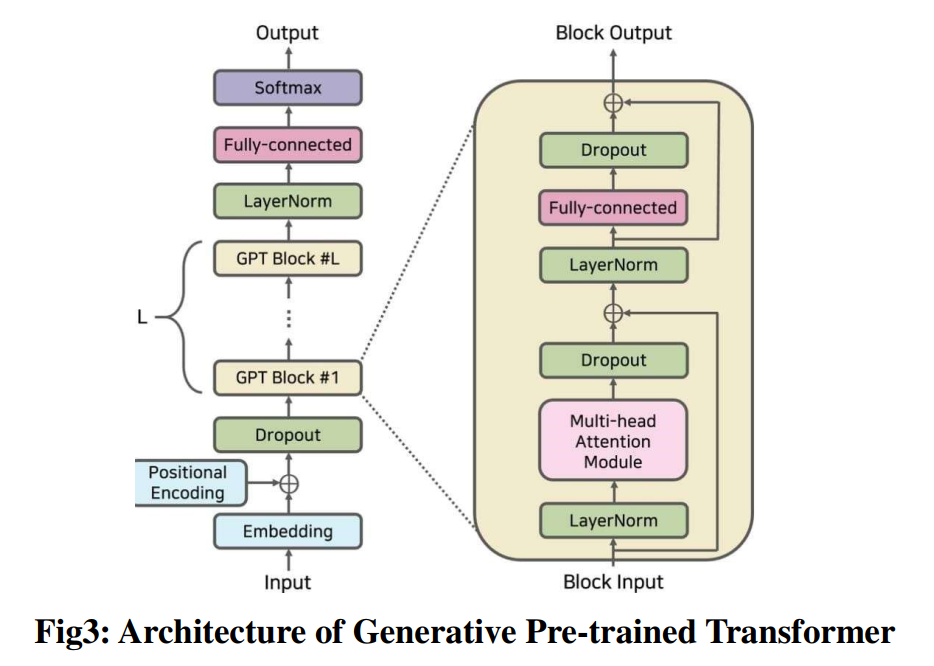
\includegraphics[width=0.8\linewidth]{img/chap04/gptstructure.png}
    \caption{Architecture of Generative Pre-trained Transformer}
    \label{fig:gptarch}
\end{figure}

    \item BERT (Bidirectional Encoder Representations from Transformers)

Released by Google in 2018, BERT revolutionized NLP by introducing a bidirectional pre-training approach. Unlike previous models that processed text sequentially, BERT leveraged masked language modelling and next sentence prediction tasks to capture contextual information bidirectionally. This enabled BERT to achieve stateof-the-art performance on a wide range of NLP tasks, including sentiment analysis, named entity recognition, and question answering.

\begin{figure}[h]
    \centering
    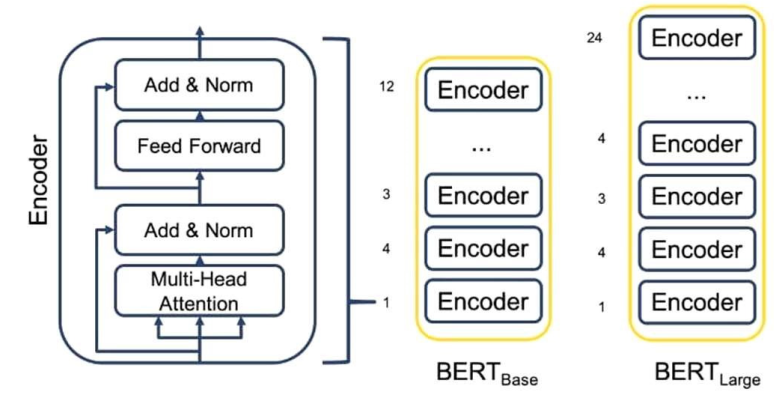
\includegraphics[width=0.8\linewidth]{img/chap04/bertarch.png}
    \caption{Bidirectional Encoder Representation from Transformer's Architecture}
    \label{bertarch}
\end{figure}

\item XLNet

Introduced by researchers at Google AI in 2019, XLNet further advanced the stateof-the-art in LLMs by addressing limitations of previous models such as token-level permutation and context fragmentation. XLNet employed a permutation-based training objective, allowing it to capture bidirectional context while maintaining the advantages of autoregressive  language modelling. This approach resulted in improved performance on various benchmark tasks, surpassing previous models like BERT.

\begin{figure}[h]
    \centering
    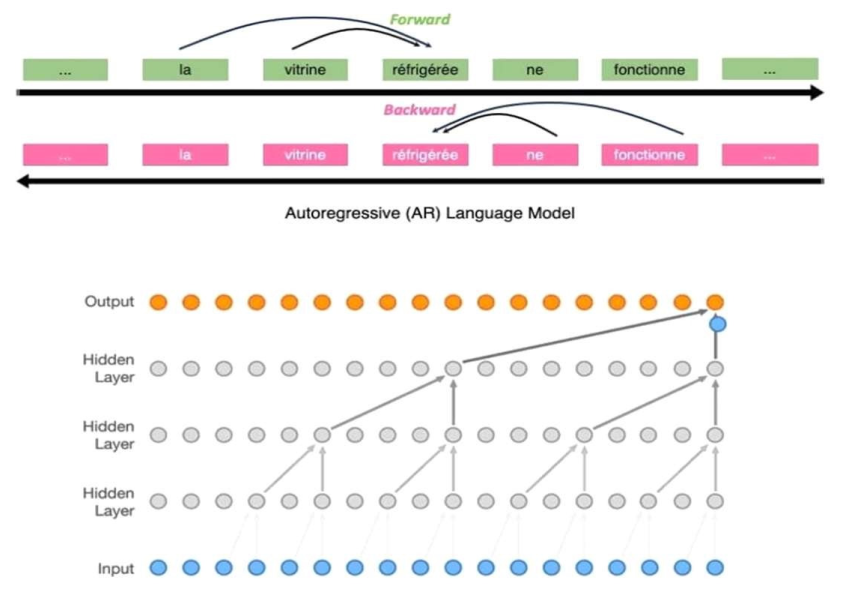
\includegraphics[width=0.8\linewidth]{img/chap04/xlnet-arch.png}
    \caption{Understanding language using XLNET with autoregressive pre-training}
    \label{fig:xlnet-arch}
\end{figure}

\item T5 (Text-To-Text Transfer Transformer)

Developed by researchers at Google AI in 2019, T5 introduced a unified framework for NLP tasks by formulating them as text-to-text transformations. Unlike traditional models that were designed for specific tasks, T5 could perform multiple tasks, including translation, summarization, question answering, and text classification, by simply altering the input-output format. This approach simplified model architecture and training, leading to more efficient and versatile LLMs.
\begin{figure}[h]
    \centering
    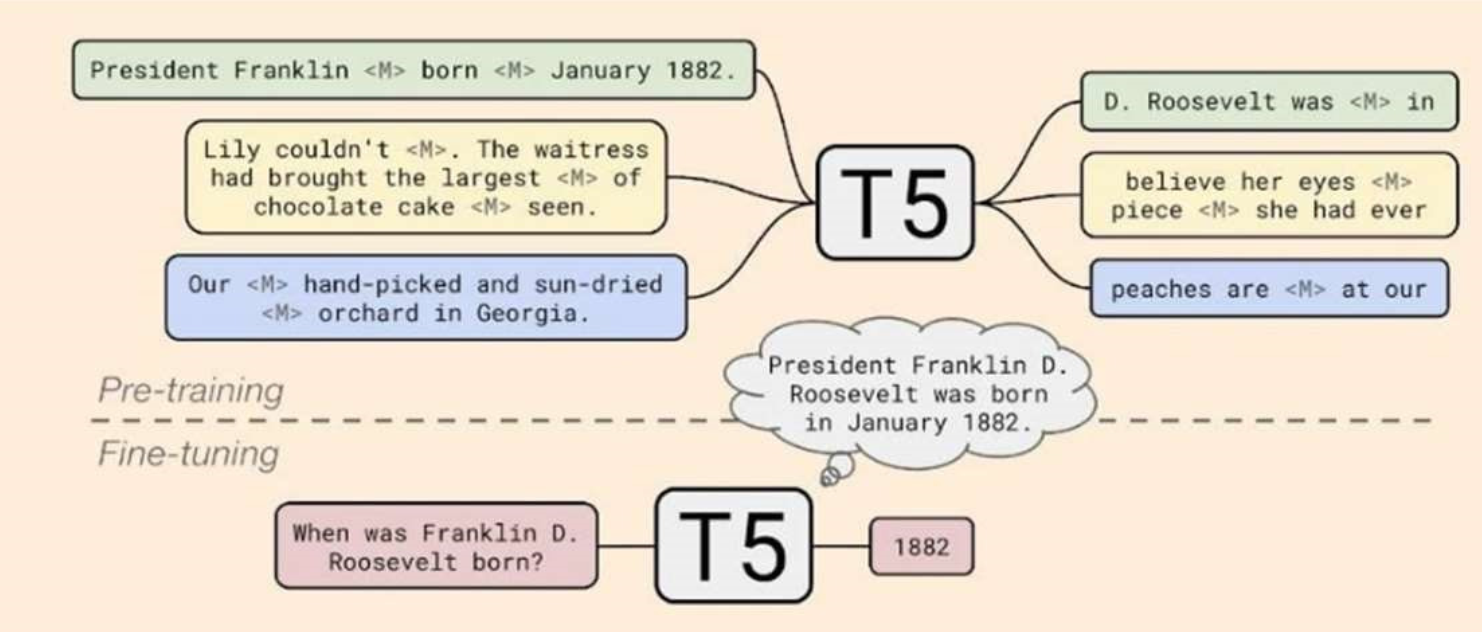
\includegraphics[width=0.8\linewidth]{img/chap04/t5arch.png}
    \caption{Google Text-to-Text Transfer Transformer(T5)}
    \label{fig:t5-arch}
\end{figure}

\end{enumerate}


\subsection{LLM Agents}

One of the bigger frontiers in LLM research is the creation of agents. ChatGPT and similar platforms can generate API calls and functioning code, but humans still need to copy and paste the code to actually do anything with it.

Agents are meant to get around this limitation. Auto-GPT, for example, pairs an underlying LLM with a “bot” that takes high-level tasks, breaks them down into tasks an LLM can solve, and stitches together those solutions. The integration of LLMs into AI agents has significantly advanced their performance, enabling more complex reasoning and decision-making processes. These agents can now autonomously navigate tasks such as web browsing, information synthesis, and report generation, effectively augmenting white-collar work. For instance, OpenAI's Deep Research agent exemplifies this progression by autonomously exploring the web, selecting pertinent information, and compiling detailed reports.

\subsection{Multimodal Models}

Another development worth mentioning is the rise of multi-modality. A model is “multi-modal” when it can process more than one kind of information, like images and text.

LLMs are staggeringly good at producing coherent language, and image models could do the same thing with images, but now a lot of time and effort is being spent on combining these two kinds of functionality.

The result has been models able to find specific sections of lengthy videos, generate images to accompany textual explanations, and create their own incredible videos from short, simple prompts.

Multimodal models extend the capabilities of traditional LLMs by integrating and processing multiple data modalities, such as text, images, audio, and video. This integration enables a more comprehensive understanding and generation of content across various formats. The progression towards Multimodal Large Language Models (MLLMs) represents a significant advancement in AI, facilitating applications that require simultaneous interpretation of diverse data types. For example, Meta's Llama 3.2 model can process visual information, enabling applications in robotics and virtual reality. 
The incorporation of multimodal capabilities into LLMs has led to models that can perform tasks such as visual grounding, image generation and editing, and comprehensive content understanding. This evolution reflects a broader trend towards creating AI systems capable of more nuanced and context-rich interactions. 

% \section{Factors Propelling the Evolution of LLMs}


% \section{\textbf{Increased Data Diversity and Volume}}


% \section{\textbf{Computational Advancements}}


% \section{\textbf{Algorithmic Innovations: The Transformer Architecture}}

% \section{Key Architectural and Training Innovations}


% \section{\textbf{The Transformer Model and Self-Attention}}


% \section{Pre-training Objectives (e.g., MLM, Prefix LM)}


% \section{Scaling Laws and Compute-Optimal Training}


% \section{Advancements in Context Length}


% \section{Techniques for Efficient Training and Inference}


% \section{Impact and Applications Across Domains}


% \section{Natural Language Processing Tasks}


% \section{Creative Work and Knowledge Work}


% \section{Science, Medicine, and Law}


% \section{Robotics and Embodied Agents}


% \section{Synthetic Data Generation}


% \section{Ongoing Challenges and Future Directions}


% \section{Behavioral Challenges (e.g., Hallucinations, Misalignment)}


% \section{Scientific Challenges (e.g., Reproducibility)}


% \section{Ethical Considerations}


% \section{Towards More Capable and Reliable LLMs}

\newpage 

\chapter{Fine-Tuning Techniques for Large Language Models}

\section{Overview of Fine-Tuning}

Large Language Models (LLMs) have demonstrated \textbf{extraordinary capabilities} in understanding, generating, and reasoning with natural language. This is largely due to their \textbf{pre-training on vast and diverse textual corpora} sourced from the internet, including books, articles, web pages, and forums. Through this process, models such as GPT, BERT, and LLaMA are able to capture a wide range of linguistic features—such as grammar, syntax, semantics—as well as broad factual and commonsense knowledge. These models operate as powerful general-purpose language processors that can be applied across a variety of tasks.

\vspace{0.5cm}

Despite these strengths, \textbf{pre-training alone is not sufficient} when it comes to achieving high performance on specialized tasks or domain-specific applications. For example, a general LLM might perform poorly on biomedical question answering, legal contract analysis, or technical customer support conversations. This limitation arises because the model, while broadly knowledgeable, may not be adequately exposed to the terminology, patterns, and nuances specific to these specialized fields during pre-training.

\vspace{0.5cm}

To bridge this gap, researchers and practitioners employ a technique known as \textbf{fine-tuning}. Fine-tuning refers to the process of \emph{continuing the training of a pre-trained model} on a smaller, curated dataset that is specific to a given task or domain. This dataset is typically labeled and reflects the desired outputs of the target application. During fine-tuning, the model adjusts its internal representations and decision boundaries to align more closely with domain-specific data, thereby improving its performance on the intended task.

\vspace{0.5cm}

Importantly, \textbf{fine-tuning enables the model to retain the general knowledge acquired during pre-training while specializing in a narrower objective}. This balance is critical: the model must not forget its foundational language capabilities, yet it must become more responsive and accurate in the new context. Tasks that benefit from fine-tuning include, but are not limited to, sentiment analysis, named entity recognition in specialized corpora (e.g., medical or financial texts), domain-specific dialogue systems, and document classification.


\vspace{1cm}

\begin{figure}[H]
    \centering
    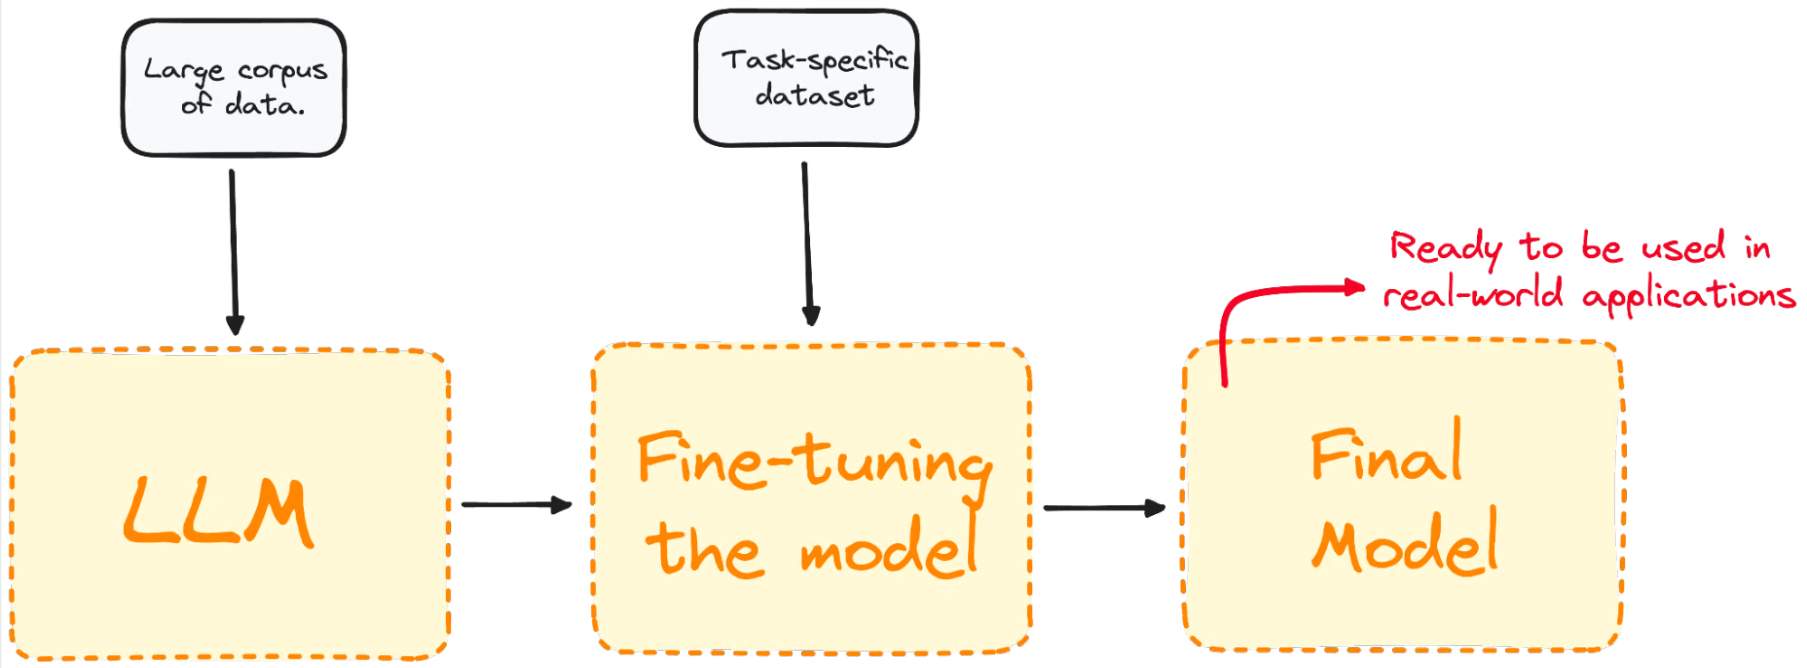
\includegraphics[width=0.95\linewidth]{img/chap05/5.1.2.png}
    \caption{From pre-trained LLM to final model ready for deployment through fine-tuning.}
    \label{fig:finetune_overview_2}
\end{figure}

\textbf{Fine-tuning is most commonly implemented using supervised learning}, in which a labeled dataset—consisting of input-output pairs specific to the target domain—is employed to guide the learning process. In this context, supervision refers to the use of explicit examples that show the model how to behave in the desired way. The objective is to refine the model’s outputs so that they become more relevant, accurate, and consistent with domain-specific expectations.

\vspace{0.5cm}

For example, a base LLM that was pre-trained on general-purpose internet text (e.g., Wikipedia, Common Crawl, news articles) may not perform optimally in specialized environments such as clinical report generation, legal document summarization, or customer service chatbots. By fine-tuning the base model on a \emph{proprietary knowledge base} or an \emph{application-specific dataset}—which may include domain-specific terminology, structured templates, or conversational patterns—the model's behavior becomes more aligned with the practical requirements of that particular context.

\vspace{0.5cm}

The \textbf{primary advantage of fine-tuning is its dual benefit}: it preserves the broad linguistic and factual knowledge acquired during the large-scale pre-training phase, while adapting the model to meet the unique demands of a specific application. This process results in a \textbf{fine-tuned model} that is more robust, task-aligned, and ready for integration into downstream systems. Such a model not only demonstrates improved quantitative performance (e.g., higher accuracy or F1 score) on the fine-tuned task but also offers greater utility in real-world deployments, where general-purpose responses may not suffice.

\vspace{0.5cm}

Figure~\ref{fig:finetune_overview_1} presents a high-level overview of this transformation pipeline: starting from a pre-trained base LLM, the model is enhanced via supervised fine-tuning on a specialized knowledge source. Likewise, Figure~\ref{fig:finetune_overview_2} illustrates a similar conceptual flow—from pre-training on a large generic corpus to targeted fine-tuning, ultimately producing a model that is \textbf{ready for deployment in real-world applications}.

\vspace{1cm}

\begin{figure}[H]
    \centering
    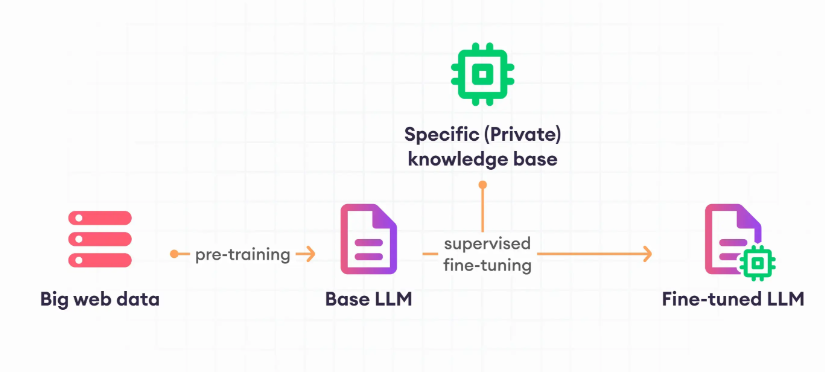
\includegraphics[width=0.85\linewidth]{img/chap05/5.1.1.png}
    \caption{Supervised fine-tuning of a base LLM using specific (possibly private) knowledge.}
    \label{fig:finetune_overview_1}
\end{figure}



\section{Types of Fine-Tuning Techniques}

\subsection{Full Fine-Tuning}
\begin{figure}[ht]
\centering
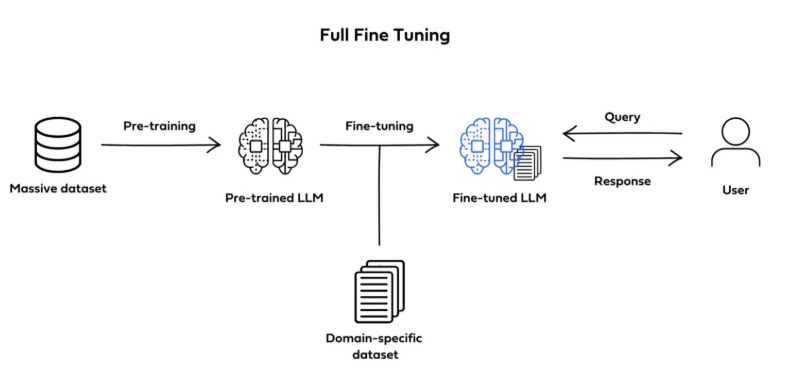
\includegraphics[width=0.9\textwidth]{img/chap05/5.2.1.png}
\caption{Illustration of the full fine-tuning process, showing how all parameters of a pre-trained LLM are updated using a domain-specific dataset to create a fine-tuned model that can handle specialized queries.}
\label{fig:full-fine-tuning}
\end{figure}

Full fine-tuning represents a comprehensive adaptation approach where \textbf{all parameters} of a pre-trained language model undergo adjustment using a task-specific or domain-specific dataset, as illustrated in Figure \ref{fig:full-fine-tuning}. This methodology leverages the foundational knowledge captured during pre-training while enabling the model to specialize for particular applications or domains.

\vspace{0.5cm}

In this approach, the entire neural network architecture—including attention mechanisms, feed-forward layers, and embedding matrices—is subjected to additional training iterations. The process begins with a pre-trained model that has already learned general language patterns and semantic relationships from massive corpora. This model serves as the initialization point for subsequent training, where every weight and bias throughout the network becomes eligible for modification.

\vspace{0.5cm}

The mechanism operates through supervised learning on labeled examples relevant to the target task. During fine-tuning, input sequences from the specialized dataset are processed through the model, generating predictions that are compared against ground truth labels. The resulting loss is backpropagated through the complete network hierarchy, and \textit{all parameters} are incrementally updated using optimization algorithms such as Adam or AdamW.

\vspace{0.5cm}

Mathematically, for each parameter $\theta_i$ in the model, updates follow the formula:
\begin{equation}
\theta_i^{new} = \theta_i^{old} - \eta \cdot \nabla_{\theta_i} \mathcal{L}
\end{equation}
where $\eta$ represents a carefully selected learning rate (typically smaller than in pre-training) and $\nabla_{\theta_i} \mathcal{L}$ denotes the gradient of the loss function with respect to parameter $\theta_i$.

\vspace{0.5cm}

To maintain stability during this process, practitioners typically implement learning rate scheduling, gradient accumulation, and normalization techniques. The learning trajectory often involves gradually decreasing the learning rate as fine-tuning progresses, allowing for initially substantial adaptations that become increasingly refined. Early stopping criteria based on validation performance help determine the optimal duration for fine-tuning iterations.

\vspace{0.5cm}

The computational workflow involves forward passes through the model for prediction generation, loss calculation against reference outputs, backward passes for gradient computation across all layers, and parameter updates according to the optimization algorithm's update rule. This cycle repeats for multiple epochs until convergence criteria are satisfied or a predetermined training budget is exhausted.

\vspace{0.5cm}

\subsection{Adapter-Based Fine-Tuning}
\begin{figure}[ht]
\centering
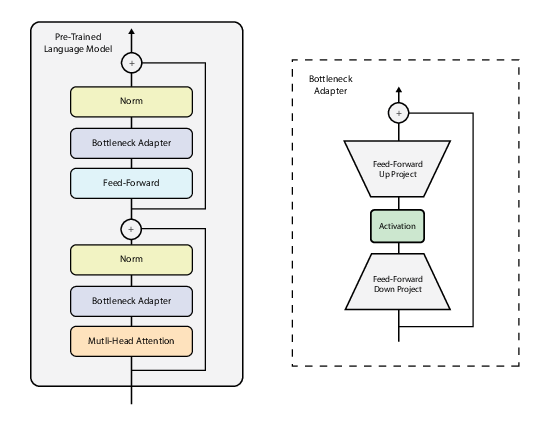
\includegraphics[width=0.9\textwidth]{img/chap05/5.2.2.png}
\caption{Architectural diagram of adapter-based fine-tuning showing the integration of bottleneck adapter modules within a pre-trained language model. The left panel illustrates adapter placement within the transformer architecture, while the right panel details the internal structure of a bottleneck adapter module.}
\label{fig:adapter-fine-tuning}
\end{figure}

Adapter-based fine-tuning represents an architectural modification approach that introduces compact, \textit{trainable neural modules}—known as adapters—into the layers of a pre-trained language model while maintaining the original model parameters in a \textbf{fixed state}. This methodology creates a parameter-efficient learning framework where only the newly inserted adapter components undergo weight updates during the adaptation process to task-specific requirements.

As depicted in Figure \ref{fig:adapter-fine-tuning}, adapter modules are strategically integrated at multiple points within the transformer architecture, typically following feed-forward networks and attention mechanisms in each layer. The fundamental structure of these adapters employs a bottleneck design that temporarily reduces dimensionality before restoring the original representation space.

\vspace{0.5cm}

The operational mechanism of an adapter module follows a three-stage computational pipeline. Initially, a down-projection matrix compresses the high-dimensional hidden representations from dimension $d$ to a significantly smaller bottleneck dimension $m$ (where $m \ll d$, often $m \approx d/64$ or smaller). Subsequently, a non-linear activation function—commonly GeLU (Gaussian Error Linear Unit) or ReLU (Rectified Linear Unit)—introduces non-linearity to the compressed representation. Finally, an up-projection matrix expands the processed features back to the original dimensionality $d$, allowing seamless integration with the surrounding network architecture.

\vspace{0.5cm}

Mathematically, for a hidden representation $h \in \mathbb{R}^d$ flowing through the network, the adapter transformation can be expressed as:

\begin{equation}
\text{Adapter}(h) = h + s \cdot (W_{\text{up}} \cdot f(W_{\text{down}} \cdot h + b_{\text{down}}) + b_{\text{up}})
\end{equation}

where $W_{\text{down}} \in \mathbb{R}^{m \times d}$ represents the down-projection matrix, $W_{\text{up}} \in \mathbb{R}^{d \times m}$ denotes the up-projection matrix, $b_{\text{down}} \in \mathbb{R}^m$ and $b_{\text{up}} \in \mathbb{R}^d$ are bias vectors, $f(\cdot)$ is the non-linear activation function, and $s$ is an optional scaling factor controlling the adapter's contribution magnitude.

\vspace{0.5cm}

The processing flow during inference or training involves the original model operations interspersed with adapter computations. Input embeddings traverse through the model's layers, with each layer's standard operations (self-attention, feed-forward networks, and normalization) occurring as designed in the pre-trained model. At designated insertion points, the adapter modules process and modify the representations through their bottleneck architecture while preserving the overall information flow via residual connections.

\vspace{0.5cm}

During the fine-tuning phase, optimization algorithms calculate gradients exclusively for the adapter parameters while treating the pre-trained model weights as constants. The learning process focuses on discovering optimal adapter configurations that effectively transform the pre-trained model's general-purpose representations into task-specialized features without altering the foundational knowledge encoded in the original parameters.

\vspace{0.5cm}

Different adapter variants may modify the precise insertion locations, bottleneck dimensionality, or employ parallel rather than sequential integration. Some implementations incorporate additional normalization layers within the adapter or utilize specialized initialization strategies to facilitate stable training dynamics.

\subsection{Low-Rank Adaptation (LoRA)}
\begin{figure}[ht]
\centering
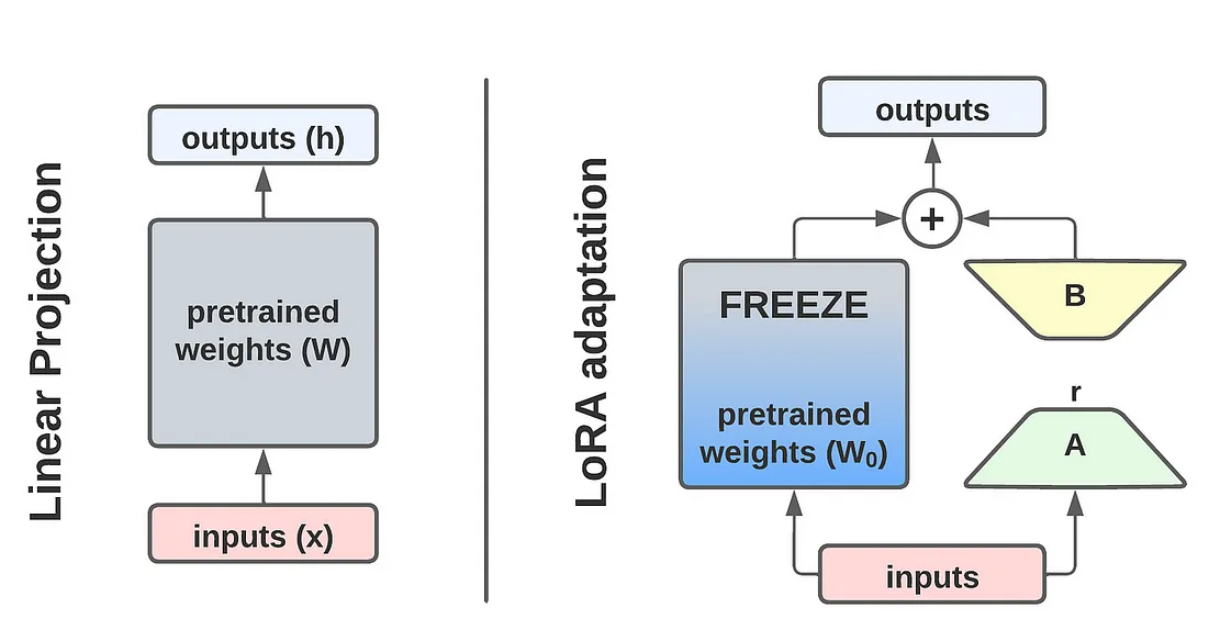
\includegraphics[width=0.9\textwidth]{img/chap05/5.2.3.png}
\caption{Comparison between standard linear projection (left) and Low-Rank Adaptation (right), illustrating how LoRA decomposes weight updates into low-rank matrices A and B that operate in parallel with frozen pre-trained weights.}
\label{fig:lora-adaptation}
\end{figure}

Low-Rank Adaptation (LoRA) represents an innovative approach to language model specialization that employs \textit{matrix decomposition principles} to enable efficient parameter updates while preserving the integrity of the original model architecture. This methodology, as depicted in Figure \ref{fig:lora-adaptation}, introduces trainable factorized matrices that operate alongside the \textbf{immutable pre-trained weights}, creating a parallel adaptation pathway.

LoRA builds upon the theoretical foundation that neural network weight updates during fine-tuning often exhibit low intrinsic dimensionality despite their high-dimensional parameterization. Rather than directly modifying the substantial weight matrices within transformer components, LoRA inserts decomposed rank-constrained matrices that capture task-specific adaptations while leaving original parameters untouched.

The mathematical formulation of LoRA centers on representing potential weight modifications through factorized low-rank structures. For a pre-trained weight matrix $W_0 \in \mathbb{R}^{d \times k}$ that would traditionally undergo updates during fine-tuning, LoRA introduces two smaller matrices: $A \in \mathbb{R}^{d \times r}$ and $B \in \mathbb{R}^{r \times k}$, where the rank hyperparameter $r$ is substantially smaller than both $d$ and $k$ (typically $r \in \{1, 2, 4, 8, 16, 32\}$). These matrices are initialized such that their product initially yields a zero contribution—$B$ is commonly initialized with zeros while $A$ uses Gaussian initialization.

During forward propagation through a LoRA-augmented network layer, the computation follows:

\begin{equation}
h' = W_0 x + \frac{\alpha}{r} A B x
\end{equation}

where $x$ represents the input activations, $h'$ denotes the output representation, $W_0$ signifies the frozen pre-trained weights, and $\alpha$ is a scaling hyperparameter that controls the magnitude of the adaptation contribution. The division by rank $r$ helps normalize the initial scale of the adapted outputs.

The learning process exclusively optimizes the parameters within matrices $A$ and $B$, leaving $W_0$ constant throughout training. Consequently, the effective update to the original transformation can be expressed as:

\begin{equation}
\Delta W = \frac{\alpha}{r} A B
\end{equation}

In practical implementations, LoRA modules are selectively applied to specific components within the transformer architecture. Most commonly, they target the query and value projection matrices within attention mechanisms, as these components heavily influence the contextual focus and information extraction capabilities of the model. Some implementations extend this approach to include key projections and feed-forward network weights, with each application following the same fundamental low-rank principle.

The computational workflow involves channeling input activations through both the original frozen pathway and the parallel LoRA pathway. The outputs from both routes are then additively combined before proceeding to subsequent operations in the network. This parallel processing structure means that during inference, the LoRA matrices can be merged with the original weights by computing $W = W_0 + \frac{\alpha}{r} A B$, enabling efficient deployment without architectural modifications.

At a system level, different LoRA modules can be trained for various tasks or domains while sharing the same underlying frozen model. The training procedure follows standard optimization approaches but isolates gradient computation and parameter updates to exclusively affect the low-rank components, maintaining the constrained adaptation space throughout the fine-tuning process.

\subsection{Prefix-Tuning}
Prefix-tuning represents an \textit{innovative} parameter-efficient fine-tuning method that modifies the behavior of a pre-trained language model by prepending a small sequence of trainable continuous vectors—called \textbf{prefix parameters}—to the input of each Transformer layer. This approach enables task-specific adaptation while keeping the underlying parameters of the language model completely \textbf{frozen}; only the prefix parameters are updated during the training process.

\begin{figure}[t]
\centering
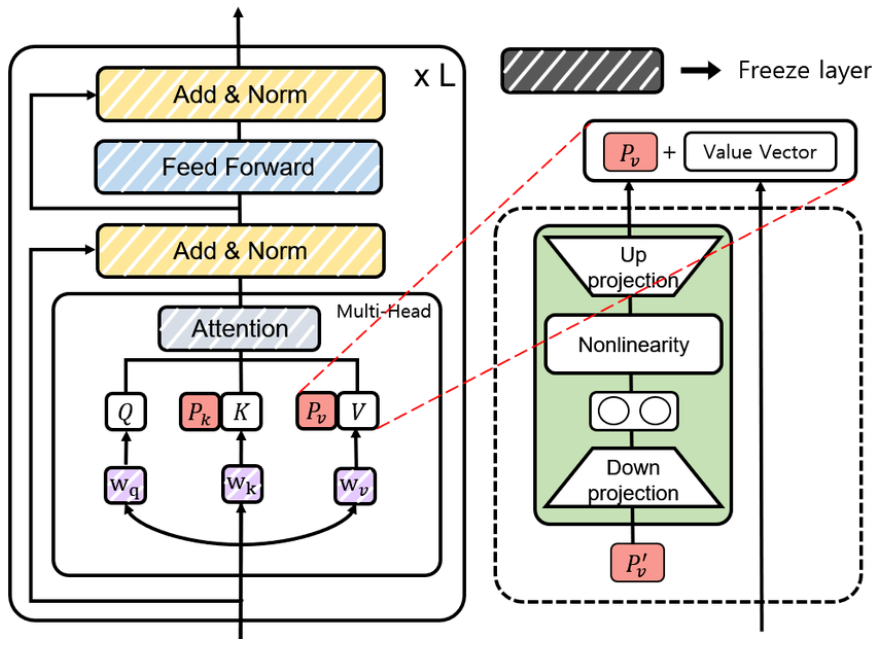
\includegraphics[width=\linewidth]{img/chap05/5.2.4.png}
\caption{Architecture of prefix-tuning. The left side shows the overall Transformer structure with attention and feed-forward blocks repeated L times. The right side illustrates the prefix mechanism, where trainable prefix vectors $P_K$ and $P_V$ are prepended to keys and values in the attention mechanism. The prefix undergoes reparameterization through a small MLP with up-projection, nonlinearity, and down-projection steps before being added to the attention computation.}
\label{fig:prefix_tuning}
\end{figure}

In the standard implementation, instead of optimizing the entire model's parameter space, prefix-tuning learns task-specific key and value vectors that are \textit{concatenated} to the original self-attention mechanism. For a Transformer block at layer \( l \), the attention computation is modified as follows:
\[
\text{Attention}(Q, [P_K^l; K], [P_V^l; V])
\]
where \( P_K^l \) and \( P_V^l \) represent the learned prefix key and value vectors for layer \( l \), and \( Q, K, V \) are the original query, key, and value matrices derived from the input tokens.

These prefix vectors function as \textbf{soft prompts}—learned continuous embeddings that effectively guide the model's behavior—without altering the model's original weights. The prefixes are typically initialized randomly and subsequently optimized using standard backpropagation techniques when trained on a supervised downstream task.

As illustrated in Figure \ref{fig:prefix_tuning}, the prefix vectors undergo a reparameterization process through a small MLP network containing an up-projection layer, a nonlinearity function, and a down-projection layer. This reparameterization helps stabilize the training dynamics and improves optimization efficiency. The resulting prefix parameters $P_K$ and $P_V$ are then prepended to the key and value matrices in the multi-head attention mechanism, effectively conditioning the model's predictions without modifying its core parameters.

The prefix-tuning mechanism operates across all layers of the Transformer architecture, with each layer receiving its own set of trainable prefix vectors. This multi-layer conditioning allows the prefixes to influence both lower-level features (in earlier layers) and higher-level semantic representations (in later layers), providing comprehensive control over the model's behavior while maintaining the underlying pre-trained knowledge intact.

\subsection{Prompt-Tuning}
Prompt-tuning represents a \textit{streamlined} and parameter-efficient fine-tuning strategy where a small number of \textbf{trainable continuous token embeddings} are prepended to the input sequence of a pre-trained language model. Unlike prefix-tuning, which modifies representations at multiple internal layers, prompt-tuning exclusively affects the initial input embedding layer, maintaining the entire underlying model architecture and parameters \textbf{completely frozen}.

\begin{figure}[t]
\centering
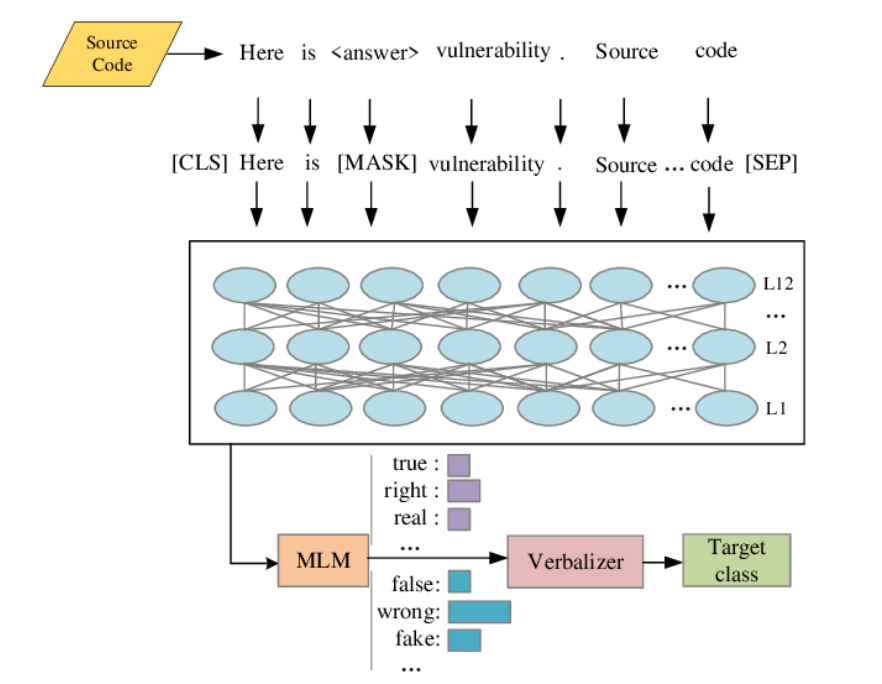
\includegraphics[width=0.8\linewidth]{img/chap05/5.2.5.png}
\caption{Architecture of prompt-tuning for classification tasks. The continuous soft prompts are prepended to tokenized inputs at the embedding layer. Special tokens like [CLS], [MASK], and [SEP] maintain their functionality while the model processes both the soft prompts and regular input through its layers (L1 through L12). The output is then processed by a masked language model (MLM) head and verbalizer to produce the target classification.}
\label{fig:prompt_tuning}
\end{figure}

In the prompt-tuning framework, the language model processes a modified input sequence represented as:
\[
[\mathbf{P}_1, \mathbf{P}_2, \ldots, \mathbf{P}_m, x_1, x_2, \ldots, x_n]
\]
where \( \mathbf{P}_i \in \mathbb{R}^d \) are the \textit{learnable} soft prompt embeddings that exist in the same dimensional space as the model's vocabulary embeddings, and \( x_i \) are the embeddings of the original input tokens. Crucially, these prompt vectors are not tied to actual vocabulary tokens but are free to occupy any position in the embedding space.

As illustrated in Figure \ref{fig:prompt_tuning}, the continuous prompt vectors are concatenated with the standard token embeddings at the input level. The combined sequence then flows through the Transformer layers (L1 through L12) without any modifications to the model architecture. The original source input undergoes tokenization with appropriate special tokens (e.g., [CLS], [MASK], [SEP] for BERT-based models) before being combined with the soft prompts.

During the training process, only the parameters of these continuous prompt embeddings are optimized, while keeping all pre-trained model weights fixed. The prompt vectors learn to elicit the desired behavior from the frozen language model through standard backpropagation based on task-specific loss functions. This creates a form of implicit conditioning that guides the model's predictions toward the target task.

For classification tasks specifically, as shown in the diagram, the processed sequence typically passes through a masked language modeling (MLM) head, followed by a verbalizer component that maps the model's vocabulary distribution to target class labels. The verbalizer establishes connections between the model's output probabilities for words like "true," "right," and "real" versus "false," "wrong," and "fake" to produce the final classification decision.

The continuous prompt embeddings are typically initialized randomly or from embeddings of template tokens and then optimized through gradient descent. The optimization process effectively discovers prompt representations that maximize task performance by leveraging the frozen model's pre-trained knowledge, allowing it to produce appropriate outputs without modifying its internal parameters.

\subsection{Instruction Tuning}
Instruction tuning is a specialized fine-tuning methodology in which a pre-trained language model undergoes additional training on a diverse collection of examples formatted as \textbf{explicit natural language directives paired with appropriate responses}. The fundamental principle involves aligning the model's behavior with human intentions by teaching it to interpret and follow clearly articulated prompts such as: \textit{"Translate the following sentence into French,"} \textit{"Summarize the paragraph below,"} or \textit{"Explain the concept of quantum computing to a high school student."} 

\begin{figure}[t]
\centering
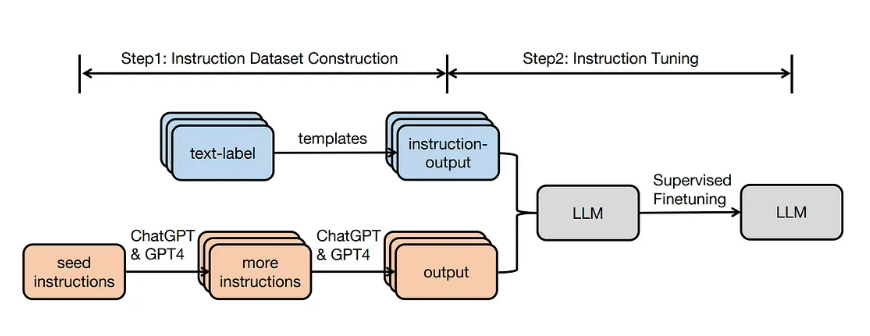
\includegraphics[width=\linewidth]{img/chap05/5.2.6.png}
\caption{The two-stage process of instruction tuning. Step 1 (left) illustrates the instruction dataset construction, where text-label templates and seed instructions are expanded using stronger models like ChatGPT and GPT-4 to generate diverse instruction-output pairs. Step 2 (right) shows the actual instruction tuning phase, where the constructed dataset is used to perform supervised fine-tuning on the target LLM.}
\label{fig:instruction_tuning}
\end{figure}

As depicted in Figure \ref{fig:instruction_tuning}, the instruction tuning process typically consists of two distinct phases: instruction dataset construction and supervised fine-tuning. In the dataset construction phase, developers create or curate a wide range of instruction-output pairs, often using larger, more capable models (such as ChatGPT and GPT-4) to generate diverse examples from seed instructions and text-label templates. This approach enables the creation of comprehensive instruction datasets spanning numerous domains and task types.

During the instruction tuning phase, the training data consists of structured \textit{(instruction, input, output)} triplets. Each training example typically follows a consistent format:
\[
\texttt{Instruction:}~\textit{Perform task X} \quad \texttt{Input:}~\textit{Relevant data or query} \quad \texttt{Output:}~\textit{Expected response}
\]
For simpler tasks, the format may be condensed to instruction-output pairs where the input is implicitly contained within the instruction itself.

In the training procedure, the model receives the concatenation of the instruction and input (when present) and is trained using standard language modeling objectives to generate the target output. This supervised learning process utilizes traditional optimization techniques such as gradient descent with cross-entropy loss, maximizing the likelihood of producing the expected responses given the instructions.

The learning mechanism enables the model to establish connections between linguistic formulations of tasks and the corresponding expected behaviors. As the model processes numerous instruction-output examples across diverse domains, it gradually develops a generalized capability to interpret new instructions—even those formulated differently from what it encountered during training—and produce appropriate responses based on its understanding of the task requirements.

Unlike parameter-efficient methods such as prompt-tuning that incorporate learned continuous embeddings, instruction tuning directly modifies the model's full parameter space through conventional fine-tuning. This comprehensive parameter update enables the model to internalize instruction-following behavior across its entire network architecture, rather than concentrating adaptations in specific components.

The instruction tuning paradigm represents a significant shift from earlier approaches that required task-specific fine-tuning or elaborate prompt engineering. By teaching models to respond appropriately to natural language instructions, this method bridges the gap between how humans communicate their intentions and how AI systems interpret and execute tasks.


\subsection{Reinforcement Learning from Human Feedback (RLHF)}
Reinforcement Learning from Human Feedback (RLHF) represents a \textit{sophisticated} multi-stage fine-tuning paradigm designed to align large language models with human preferences and values. Unlike conventional training approaches that rely exclusively on supervised learning with predefined datasets, RLHF incorporates direct human evaluations into the optimization process, enabling models to generate outputs that better reflect human judgments of quality, helpfulness, and appropriateness.

\begin{figure}[t]
\centering
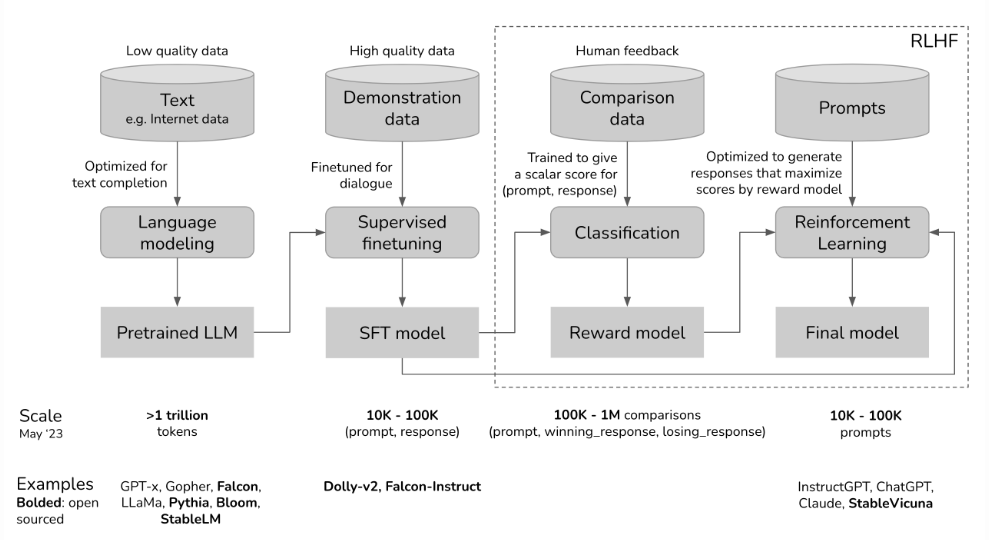
\includegraphics[width=\linewidth]{img/chap05/5.2.7.png}
\caption{Complete RLHF training pipeline. The process begins with pretraining on large text corpora (left), followed by supervised fine-tuning on demonstration data. The RLHF-specific components (outlined by the dashed box) include reward model training from human comparison data and reinforcement learning optimization. The figure also shows typical data scales for each stage and examples of models that have used these techniques.}
\label{fig:rlhf_pipeline}
\end{figure}

As illustrated in Figure \ref{fig:rlhf_pipeline}, the RLHF methodology consists of a sequential pipeline with several distinct phases, each building upon the previous one:

\begin{enumerate}
    \item \textbf{Supervised Fine-Tuning (SFT):} The process begins with a pre-trained language model that has already acquired broad linguistic capabilities through exposure to vast amounts of text data (typically exceeding 1 trillion tokens). This foundation model undergoes initial adaptation through supervised fine-tuning on a curated dataset of \textit{high-quality demonstrations}—typically comprising 10,000 to 100,000 prompt-response pairs. These examples often consist of carefully crafted responses that exhibit desirable characteristics such as helpfulness, accuracy, and safety. The resulting SFT model serves as the starting point for subsequent preference-based optimization.
    
    \item \textbf{Reward Model Development:} In this critical stage, a separate \textbf{evaluative model} is trained to predict human preferences regarding language model outputs. Human annotators are presented with a prompt and multiple alternative responses (typically generated by the SFT model) and asked to rank or compare them based on quality criteria. These comparative judgments—ranging from 100,000 to 1 million comparisons—form a specialized dataset of triplets (prompt, winning\_response, losing\_response) or (prompt, response, score). The reward model learns to assign scalar values to responses that correlate with human preferences, essentially distilling human judgments into a computational form that can guide optimization.
    
    \item \textbf{Reinforcement Learning Optimization:} The final phase leverages the trained reward model to further refine the SFT model through reinforcement learning techniques—most commonly \textit{Proximal Policy Optimization (PPO)}. During this process, the language model (now functioning as a policy) generates responses to a diverse set of prompts (typically 10,000 to 100,000). Each generated response receives a scalar reward score from the reward model, which serves as the optimization signal. The language model parameters are iteratively updated to maximize these reward scores while maintaining reasonable proximity to the original SFT model to preserve linguistic capabilities and prevent pathological optimization behaviors.
\end{enumerate}

From a mathematical perspective, the reinforcement learning objective can be formulated as maximizing:
\[
\mathbb{E}_{y \sim \pi_\phi(y|x)}[R_\theta(x, y) - \beta \log(\pi_\phi(y|x)/\pi_{\text{SFT}}(y|x))]
\]
where \( \pi_\phi \) represents the policy (language model) being optimized with parameters \( \phi \), \( R_\theta \) denotes the reward model with parameters \( \theta \), \( x \) is the input prompt, \( y \) is the generated response, and \( \pi_{\text{SFT}} \) is the initial supervised fine-tuned model. The second term—controlled by the hyperparameter \( \beta \)—constitutes a KL-divergence penalty that prevents the optimized model from deviating too drastically from the SFT model.

The RLHF framework essentially creates a feedback loop where human preferences guide model optimization through an automated reward mechanism. This methodology enables language models to generate responses that increasingly align with human expectations and values across a diverse range of tasks and interactions. By incorporating direct human feedback into the training process, RLHF addresses fundamental challenges in specifying complex objectives that are difficult to articulate through conventional loss functions or supervised learning approaches alone.

\section{Advantages and Disadvantages of Fine-Tuning Methods}

\subsection{Full Fine-Tuning}

Full fine-tuning involves updating all parameters of a pre-trained language model when adapting it to a downstream task. This comprehensive approach offers distinct trade-offs that practitioners should consider.

\subsubsection{Advantages}
\begin{itemize}
    \item \textbf{Superior Performance}: Generally achieves the highest task-specific performance compared to parameter-efficient methods, as all model weights can adapt to the target domain.
    \item \textbf{Complete Representation Learning}: Allows modification of features at all levels of abstraction throughout the network hierarchy.
    \item \textbf{Robust Transfer}: Can effectively adapt to domains significantly different from pre-training data by thoroughly rewriting relevant representations.
    \item \textbf{Flexibility}: Imposes no architectural constraints on adaptation, enabling unrestricted optimization.
\end{itemize}

\subsubsection{Disadvantages}
\begin{itemize}
    \item \textbf{Resource Intensity}: Requires substantial computational resources (GPU/TPU memory and compute) proportional to the model size.
    \item \textbf{Storage Overhead}: Each fine-tuned variant requires storing a complete copy of model parameters, creating significant storage costs for large models.
    \item \textbf{Catastrophic Forgetting}: Models may lose general capabilities and knowledge acquired during pre-training when aggressively optimized on narrow tasks.
    \item \textbf{Overfitting Risk}: Higher susceptibility to overfitting on smaller datasets due to the large number of trainable parameters.
\end{itemize}

\subsubsection{Practical Considerations}
Full fine-tuning is most appropriate when maximum task performance is the primary objective and sufficient computational resources are available. Consider alternatives when facing computational constraints or working with limited datasets. For implementation, use smaller learning rates than during pre-training (typically 1e-5 to 1e-6), apply appropriate regularization techniques, and monitor for signs of catastrophic forgetting. Mixed-precision training and gradient checkpointing can help reduce memory requirements for larger models.

\subsection{Adapter-Based Fine-Tuning}

Adapter-based fine-tuning introduces small, trainable modules (adapters) between layers of a pre-trained language model while keeping the original parameters frozen. This parameter-efficient approach offers a distinct set of trade-offs for downstream task adaptation.

\subsubsection{Advantages}
\begin{itemize}
\item \textbf{Parameter Efficiency}: Only a small fraction of parameters (typically 1-4% of the full model) are trainable, drastically reducing memory requirements.
\item \textbf{Modular Design}: Enables easy swapping of task-specific adapters without modifying the base model, facilitating multi-task learning.
\item \textbf{Preserved Pretrained Knowledge}: The frozen base model retains its original capabilities, minimizing catastrophic forgetting.
\item \textbf{Scalability}: Particularly effective for very large models where full fine-tuning would be prohibitive.
\item \textbf{Fast Deployment}: Multiple adapters can be stored and loaded efficiently compared to full model copies.
\end{itemize}

\subsubsection{Disadvantages}
\begin{itemize}
\item \textbf{Performance Trade-off}: May achieve slightly lower task performance compared to full fine-tuning, particularly on complex tasks.
\item \textbf{Architectural Constraints}: Requires careful design of adapter placement and dimensionality within the network.
\item \textbf{Inference Overhead}: Introduces additional computational layers during forward passes, though typically minimal.
\item \textbf{Task-Specialization Limits}: May struggle with domain shifts that require deeper modifications to base representations.
\end{itemize}

\subsubsection{Practical Considerations}
Adapter-based approaches are ideal when computational resources are limited, when preserving base model capabilities is crucial, or when managing multiple task-specific versions. Optimal implementation involves:
\begin{itemize}
\item Strategic placement of adapters (typically after attention and FFN layers)
\item Careful tuning of adapter dimensionality (bottleneck size)
\item Potential combination with prefix tuning or other parameter-efficient methods
\item Use of adapter composition techniques for multi-task scenarios
\end{itemize}
Recent variants like \texttt{LoRA} (Low-Rank Adaptation) and parallel adapters offer additional design choices worth considering based on specific application requirements.

\subsection{Low-Rank Adaptation (LoRA)}

Low-Rank Adaptation (LoRA) is a parameter-efficient fine-tuning method that injects trainable low-rank matrices into a pre-trained model while keeping the original weights frozen. This approach achieves efficient adaptation with minimal memory overhead by decomposing weight updates into low-rank components.

\subsubsection{Advantages}
\begin{itemize}
    \item \textbf{Parameter Efficiency}: Updates only a small subset of parameters (typically <1\% of the full model), drastically reducing memory and storage costs while avoiding the need to store multiple full-model checkpoints.
    
    \item \textbf{No Inference Latency}: Unlike adapters, LoRA can be merged with the original weights after training, introducing zero additional computation during inference.
    
    \item \textbf{Preserved Pretrained Knowledge}: The base model remains frozen, minimizing catastrophic forgetting and enabling switching between different task-specific LoRA modules without reloading the base model.
    
    \item \textbf{Scalability}: Particularly effective for fine-tuning large language models (LLMs) where full fine-tuning is impractical, and compatible with quantization techniques for further efficiency gains.
    
    \item \textbf{Flexibility}: Can be applied selectively to specific layers (e.g., attention weights only) for targeted adaptation.
\end{itemize}

\subsubsection{Disadvantages}
\begin{itemize}
    \item \textbf{Performance Trade-off}: May underperform full fine-tuning on tasks requiring deep architectural changes due to the low-rank constraint limiting update expressiveness.
    
    \item \textbf{Rank Selection Sensitivity}: Performance depends on choosing an appropriate rank for the decomposition (too low leads to weak adaptation, too high has diminishing returns).
    
    \item \textbf{Task-Specific Tuning Required}: Optimal rank and layer selection may vary across tasks, requiring experimentation.
    
    \item \textbf{Limited Extreme Domain Adaptation}: Less effective than full fine-tuning for highly specialized domains needing fundamental representation changes.
\end{itemize}

\subsubsection{Practical Considerations}
LoRA is best suited when:
\begin{itemize}
    \item Resource efficiency is a priority (e.g., fine-tuning on consumer-grade GPUs)
    \item Multiple task-specific adaptations need efficient storage and deployment
    \item Minimal inference overhead is required
\end{itemize}


\subsection{Prefix-Tuning}

Prefix-tuning is a parameter-efficient fine-tuning method that prepends trainable continuous vectors (prefixes) to the hidden states in transformer layers while keeping the original model parameters frozen. This approach provides task-specific adaptation through learned "soft prompts" that condition the model's behavior.

\subsubsection{Advantages}
\begin{itemize}
    \item \textbf{Extreme Parameter Efficiency}: Only requires training of a small prefix (typically 0.1-1\% of model parameters), making it highly memory-efficient.
    
    \item \textbf{Architectural Preservation}: Maintains the original model architecture without modifications, ensuring no inference overhead after deployment.
    
    \item \textbf{Multi-Task Flexibility}: Different prefixes can be swapped in/out at runtime, enabling efficient multi-task serving from a single base model.
    
    \item \textbf{Knowledge Retention}: Frozen base model parameters prevent catastrophic forgetting of pre-trained knowledge.
    
    \item \textbf{Discrete Prompt Generalization}: Outperforms manual prompt engineering by learning optimal continuous prefixes.
\end{itemize}

\subsubsection{Disadvantages}
\begin{itemize}
    \item \textbf{Sequence Length Impact}: Added prefix tokens reduce the available context window for the actual input.
    
    \item \textbf{Optimization Challenges}: Requires careful tuning of prefix length and learning rates due to the discrete nature of the approach.
    
    \item \textbf{Performance Trade-offs}: May underperform full fine-tuning on complex tasks requiring deep architectural changes.
    
    \item \textbf{Layer Placement Sensitivity}: Performance varies significantly based on which transformer layers receive prefixes.
\end{itemize}

\subsubsection{Practical Considerations}
Prefix-tuning is most appropriate when parameter efficiency and model preservation are prioritized over absolute task performance, particularly in resource-constrained environments or multi-task scenarios. Consider alternative methods when working with tasks requiring fundamental architectural changes or when the prefix length would excessively reduce the available context window. For implementation, use moderate learning rates (typically 1e-4 to 1e-5) given the discrete nature of prefix optimization, apply layer normalization to the prefixes for training stability, and carefully tune the prefix length based on task complexity. Techniques like gradient clipping and weight decay are particularly important for successful optimization. The approach works especially well when combined with prompt-based fine-tuning paradigms.

\subsection{Prompt-Tuning}

Prompt-tuning is a parameter-efficient approach that learns continuous "soft" prompts while keeping the entire pre-trained model frozen. Unlike traditional prompt engineering, it automatically optimizes task-specific embeddings prepended to the input sequence.

\subsubsection{Advantages}
\begin{itemize}
    \item \textbf{Extreme Efficiency}: Only requires training the prompt parameters (typically <0.1\% of model parameters), making it highly resource-friendly.
    
    \item \textbf{No Architecture Changes}: Preserves the original model structure without adding new layers or modules.
    
    \item \textbf{Multi-Task Deployment}: Enables serving multiple tasks from a single frozen model by switching learned prompts.
    
    \item \textbf{Knowledge Preservation}: Maintains all original model capabilities as base parameters remain frozen.
    
    \item \textbf{Superior to Manual Prompts}: Outperforms hand-crafted discrete prompts through learned continuous representations.
\end{itemize}

\subsubsection{Disadvantages}
\begin{itemize}
    \item \textbf{Context Window Reduction}: Learned prompts consume part of the available sequence length.
    
    \item \textbf{Task Complexity Limitations}: Less effective for tasks requiring substantial model adaptation beyond input conditioning.
    
    \item \textbf{Optimization Sensitivity}: Requires careful tuning of prompt length and learning rates.
    
    \item \textbf{Performance Gap}: Generally underperforms full fine-tuning on complex downstream tasks.
\end{itemize}

\subsubsection{Practical Considerations}
Prompt-tuning is most suitable when working with very large models where parameter efficiency is crucial, or when maintaining the base model's general capabilities is essential. Consider alternative methods when dealing with tasks that require significant architectural changes or when the performance gap is unacceptable. For implementation, use relatively high learning rates (typically 1e-3 to 1e-4) due to the small parameter count, initialize prompts from relevant word embeddings when possible, and experiment with prompt lengths between 20-100 tokens based on task complexity. The approach works particularly well when combined with few-shot learning paradigms.

\subsection{Instruction Tuning}

Instruction tuning is a supervised fine-tuning approach that trains language models on diverse tasks formatted with natural language instructions, enabling zero-shot generalization to unseen tasks. This method focuses on teaching models to follow task specifications rather than specializing for particular datasets.

\subsubsection{Advantages}
\begin{itemize}
    \item \textbf{Zero-shot Generalization}: Enables models to perform unseen tasks by following natural language instructions without task-specific fine-tuning.
    
    \item \textbf{Task Formulation Flexibility}: Handles diverse tasks through standardized instruction-input-output formatting.
    
    \item \textbf{Human-Aligned Behavior}: Produces more interpretable and controllable outputs by conditioning on explicit instructions.
    
    \item \textbf{Multi-Task Efficiency}: Single instruction-tuned model can replace multiple specialized models.
    
    \item \textbf{Knowledge Preservation}: Maintains broad capabilities from pre-training while adding instruction-following skills.
\end{itemize}

\subsubsection{Disadvantages}
\begin{itemize}
    \item \textbf{Data Requirements}: Needs large, diverse collections of instruction-output pairs covering various task types.
    
    \item \textbf{Training Cost}: Requires substantial computational resources comparable to full fine-tuning.
    
    \item \textbf{Instruction Sensitivity}: Performance heavily depends on how tasks are formulated in natural language.
    
    \item \textbf{Over-optimization Risk}: May lose general capabilities if tuned too aggressively on narrow instruction sets.
\end{itemize}

\subsubsection{Practical Considerations}
Instruction tuning is most valuable when building general-purpose models that need to handle diverse, unpredictable tasks through natural language interaction. It becomes particularly effective when paired with large language models that have sufficient capacity to internalize the instruction-following paradigm. The approach requires careful curation of training tasks to ensure broad coverage of potential use cases, with special attention to the variety and clarity of instruction formulations. While powerful for zero-shot applications, performance on specific tasks may still lag behind specialized fine-tuned models, making the technique better suited for general assistants than domain-specific applications where peak performance is required.

\subsection{Reinforcement Learning from Human Feedback (RLHF)}

RLHF is an alignment technique that uses reinforcement learning to fine-tune language models based on human preferences, typically through a reward model trained on human judgments. This approach bridges the gap between raw language model capabilities and human-desirable behaviors.

\subsubsection{Advantages}
\begin{itemize}
    \item \textbf{Human-Aligned Outputs}: Produces responses better aligned with human values and preferences compared to supervised fine-tuning alone.
    
    \item \textbf{Complex Behavior Shaping}: Can optimize for nuanced aspects of responses (e.g., helpfulness, harmlessness) that are difficult to specify explicitly.
    
    \item \textbf{Adaptability}: Capable of learning from relatively small amounts of human preference data compared to the original training data.
    
    \item \textbf{Multi-Dimensional Optimization}: Enables balancing of competing objectives through reward modeling.
    
    \item \textbf{Iterative Improvement}: Supports continuous refinement of model behavior through additional feedback rounds.
\end{itemize}

\subsubsection{Disadvantages}
\begin{itemize}
    \item \textbf{Implementation Complexity}: Requires sophisticated pipeline with reward modeling and RL optimization components.
    
    \item \textbf{High Resource Demands}: Needs substantial compute for both reward model training and RL fine-tuning phases.
    
    \item \textbf{Reward Hacking Risk}: Models may exploit weaknesses in the reward model rather than genuinely improving.
    
    \item \textbf{Data Bottleneck}: Quality heavily depends on the quantity and diversity of human preference data.
    
    \item \textbf{Instability}: RL training can be unpredictable and sensitive to hyperparameters.
\end{itemize}

\subsubsection{Practical Considerations}
RLHF is most valuable when aligning large language models to complex human preferences where simple supervised approaches are insufficient. The technique proves particularly effective for refining safety properties and conversational abilities, but requires careful implementation to avoid reward gaming behaviors. Significant investment in high-quality human preference data collection is essential, and the approach works best when combined with initial supervised fine-tuning as a foundation. While powerful, RLHF should be deployed judiciously due to its computational demands and implementation complexity, making it most suitable for foundational models rather than application-specific tuning.

\newpage 

\chapter{Code Engineering}

\section{Fine-Tuning Results Comparison}

\subsection{Overview of Experimental Settings}

To investigate the effectiveness of various fine-tuning techniques on large language models (LLMs), we conducted a comprehensive evaluation involving three transformer-based models: \textbf{T5-base}, \textbf{BART-base}, and \textbf{Flan-T5-small}. Each model was fine-tuned using three distinct methods: \textbf{Full Finetuning}, \textbf{Low-Rank Adaptation (LoRA)}, and \textbf{Adapters}. These fine-tuning strategies were applied across three representative NLP tasks—\textbf{Question Answering}, \textbf{Machine Translation}, and \textbf{Sentiment Classification}—chosen to cover a range of language understanding capabilities.

\subsection{Evaluation Criteria}

Each task provides multiple metrics for evaluation; however, to maintain a consistent and interpretable comparison across different methods and models, we select a primary metric for each task based on its relevance and widespread usage:

\begin{itemize}
    \item For \textbf{Question Answering (SQuAD 1.0)}, we focus on the \textbf{F1 Score}, which captures both precision and recall, and is especially important for extractive QA tasks.
    \item For \textbf{Translation (WMT16 English-German)}, we use the \textbf{BLEU Score}, a standard metric that quantifies translation quality based on n-gram overlap with reference translations.
    \item For \textbf{Sentiment Classification (IMDB)}, we again rely on the \textbf{F1 Score}, as it provides a balanced measure of classification performance in the presence of potential label imbalance.
\end{itemize}

\subsection{Best Performing Configurations}

\begin{table}[H]
    \centering
    \begin{tabular}{|>{\centering\arraybackslash}m{3cm}|>{\centering\arraybackslash}m{3cm}|>{\centering\arraybackslash}m{3cm}|>{\centering\arraybackslash}m{3cm}|}
    \hline
    \textbf{Model} & \textbf{Method} & \textbf{BLEU Score} & \textbf{Cosine Similarity} \\
    \hline
    \multirow{3}{*}{T5-base} 
    & Full Finetuning & 0.2259 & 0.4400 \\
    & LoRA             & 0.1999 & 0.3812 \\
    & Adapters         & 0.2355 & 0.4256 \\
    \hline
    \multirow{3}{*}{BART-base} 
    & Full Finetuning & 0.1197 & 0.3499 \\
    & LoRA             & 0.0491 & 0.2423 \\
    & Adapters         & 0.0001 & 0.0642 \\
    \hline
    \multirow{3}{*}{Flan-T5-small} 
    & Full Finetuning & 0.1383 & 0.3559 \\
    & LoRA             & 0.0762 & 0.2807 \\
    & Adapters         & 0.1095 & 0.3287 \\
    \hline
    \end{tabular}
    \caption{Translation}
\end{table}
    
\begin{table}[H]
    \centering
    \begin{tabular}{|>{\centering\arraybackslash}m{3cm}|>{\centering\arraybackslash}m{3cm}|>{\centering\arraybackslash}m{3cm}|>{\centering\arraybackslash}m{3cm}|}
    \hline
    \textbf{Model} & \textbf{Method} & \textbf{Exact Match (EM)} & \textbf{F1 Score} \\
    \hline
    \multirow{3}{*}{T5-base} 
    & Full Finetuning & 85.2312\% & 87.3847\% \\
    & LoRA             & 94.3136\% & 95.7342\% \\
    & Adapters         & 92.6941\% & 94.4193\% \\
    \hline
    \multirow{3}{*}{BART-base} 
    & Full Finetuning & 69.3850\% & 73.6033\% \\
    & LoRA             & 84.1681\% & 87.0804\% \\
    & Adapters         & 36.5725\% & 40.9718\% \\
    \hline
    \multirow{3}{*}{Flan-T5-small} 
    & Full Finetuning & 82.5057\% & 84.9403\% \\
    & LoRA             & 74.2509\% & 76.9574\% \\
    & Adapters         & 84.1039\% & 86.3504\% \\
    \hline
    \end{tabular}
    \caption{Question Answering}
\end{table}
    
\begin{table}[H]
    \centering
    \begin{tabular}{|>{\centering\arraybackslash}m{3cm}|>{\centering\arraybackslash}m{3cm}|>{\centering\arraybackslash}m{2cm}|>{\centering\arraybackslash}m{2cm}|>{\centering\arraybackslash}m{2cm}|>{\centering\arraybackslash}m{2cm}|}
    \hline
    \textbf{Model} & \textbf{Method} & \textbf{Accuracy} & \textbf{Precision} & \textbf{Recall} & \textbf{F1 Score} \\
    \hline
    \multirow{3}{*}{T5-base} 
    & Full Finetuning & 0.9425 & 0.9667 & 0.9239 & 0.9449 \\
    & LoRA            & 0.7063 & 0.7029 & 0.7335 & 0.7179 \\
    & Adapters        & 0.9084 & 0.8946 & 0.9298 & 0.9119 \\
    \hline
    \multirow{3}{*}{BART-base} 
    & Full Finetuning & 0.9021 & 0.8942 & 0.9163 & 0.9051 \\
    & LoRA            & 0.9184 & 0.9274 & 0.9112 & 0.9192 \\
    & Adapters        & 0.6074 & 0.5744 & 0.8853 & 0.6967 \\
    \hline
    \multirow{3}{*}{Flan-T5-small} 
    & Full Finetuning & 0.9142 & 0.9137 & 0.9183 & 0.9160 \\
    & LoRA            & 0.9425 & 0.9667 & 0.9239 & 0.9449 \\
    & Adapters        & 0.8895 & 0.8582 & 0.9380 & 0.8963 \\
    \hline
    \end{tabular}
    \caption{Text Sentiment}
\end{table}

The results indicate that different combinations of models and fine-tuning methods yield optimal performance depending on the task. Below, we summarize the best-performing configuration for each task based on the selected metric:

\begin{itemize}
    \item \textbf{Question Answering}: The highest F1 Score was achieved by \textbf{T5-base fine-tuned using LoRA}, reaching \textbf{95.73\%}. This suggests that LoRA is highly effective in enabling parameter-efficient learning while maintaining strong performance on extractive QA.
    
    \item \textbf{Translation}: The best BLEU Score was obtained by \textbf{T5-base with Adapters}, achieving \textbf{0.2355}. This highlights the capability of adapter-based tuning to support generative tasks like translation with competitive results while reducing the need for full model updates.
    
    \item \textbf{Sentiment Classification}: Both \textbf{T5-base with Full Finetuning} and \textbf{Flan-T5-small with LoRA} attained the top F1 Score of \textbf{0.9449}, indicating that both full parameter updates and efficient low-rank adaptation can be viable strategies for binary classification tasks.
\end{itemize}

These findings demonstrate that no single method dominates across all tasks; rather, the effectiveness of a fine-tuning strategy depends heavily on the model architecture and the nature of the downstream task. Notably, \textbf{T5-base} consistently appears in the best-performing combinations, reflecting its versatility and robustness across different NLP domains.

For more detailed comparison, key insigts and conclusion, we would say in the next part.

\newpage 

\section{Insights and Conclusion}

This section presents a comprehensive analysis of the experimental results obtained from fine-tuning three transformer-based models: \textbf{T5-base}, \textbf{BART-base}, and \textbf{Flan-T5-small}. Each model was fine-tuned on three natural language processing (NLP) tasks—\textbf{Question Answering}, \textbf{Machine Translation}, and \textbf{Sentiment Classification}—using three techniques: \textbf{Full Finetuning}, \textbf{LoRA (Low-Rank Adaptation)}, and \textbf{Adapter Tuning}.

\subsection*{1. Question Answering (SQuAD 1.0)}
\textbf{Metrics Used:} Exact Match (EM), F1 Score

\textbf{Key Observations:}
\begin{itemize}
    \item For the \textbf{T5-base} model, \textbf{LoRA} achieved the highest performance among all configurations, with an EM of 94.31\% and F1 of 95.73\%. This result surpasses both full finetuning and adapter tuning, indicating that LoRA can efficiently capture task-relevant information with fewer trainable parameters.
    
    \item The \textbf{Adapter} approach also performs competitively on T5-base (EM: 92.69\%, F1: 94.42\%), making it a lightweight yet strong alternative to full finetuning.
    
    \item \textbf{BART-base} shows mixed results. While LoRA improves performance significantly over full finetuning (EM from 69.38\% to 84.17\%), adapter tuning fails catastrophically (EM: 36.57\%, F1: 40.97\%), suggesting that adapter layers are not well-aligned with BART’s architecture for QA tasks.
    
    \item \textbf{Flan-T5-small} exhibits a noteworthy trend where adapter tuning (F1: 86.35\%) outperforms full finetuning (F1: 84.94\%). This suggests that smaller, instruction-tuned models may be more amenable to modular fine-tuning techniques.
\end{itemize}

\textbf{Conclusion:} 
\textbf{LoRA stands out as the best method for question answering}, particularly with T5-based models, achieving both high accuracy and computational efficiency. Adapter tuning also performs well on encoder-decoder models like T5, but its application on BART requires further investigation due to poor compatibility. Interestingly, even small models like \textbf{Flan-T5-small} can rival larger ones when equipped with suitable fine-tuning techniques.

\subsection*{2. Machine Translation (WMT16 English-German)}
\textbf{Metrics Used:} BLEU Score, Cosine Similarity

\textbf{Key Observations:}
\begin{itemize}
    \item \textbf{T5-base} consistently performs the best across all tuning methods in translation tasks. Notably, \textbf{Adapter tuning slightly outperforms full finetuning} in BLEU score (0.2355 vs. 0.2259), showing its strength in modular and efficient learning.
    
    \item \textbf{BART-base} performs the worst across all methods, with BLEU dropping to nearly zero with adapters (0.0001). This performance collapse suggests that the translation capabilities of BART may not generalize well under parameter-efficient tuning.
    
    \item \textbf{Flan-T5-small} delivers moderate results, with full finetuning achieving the best outcome for this model (BLEU: 0.1383). Adapter and LoRA tuning both yield subpar results compared to T5-base, likely due to the model’s smaller capacity and lack of extensive multilingual pretraining.
\end{itemize}

\textbf{Conclusion:} 
In translation tasks, \textbf{T5-base with Adapters is surprisingly the most effective}, combining high BLEU scores with modular training benefits. LoRA does not perform well for sequence generation tasks, possibly due to its limited expressiveness in controlling decoder behavior. \textbf{BART-base exhibits structural limitations for parameter-efficient methods}, making it unsuitable for lightweight translation fine-tuning without architectural modifications.

\subsection*{3. Sentiment Classification (IMDB)}
\textbf{Metrics Used:} Accuracy, Precision, Recall, F1 Score

\textbf{Key Observations:}
\begin{itemize}
    \item \textbf{T5-base with full finetuning} attains the highest performance overall (F1: 0.9449), demonstrating its capability to learn detailed classification boundaries with end-to-end training.
    
    \item \textbf{Flan-T5-small with LoRA} astonishingly matches the performance of T5-base full finetuning (F1: 0.9449). This indicates that even small models can be powerful classifiers when equipped with efficient tuning techniques like LoRA.
    
    \item \textbf{BART-base with LoRA} shows better performance than its full finetuning variant (F1: 0.9192 vs. 0.9051), suggesting that LoRA enhances generalization in this model.
    
    \item Adapters on \textbf{BART-base} again perform poorly (F1: 0.6967), reinforcing the incompatibility observed in the QA task. In contrast, \textbf{T5-base and Flan-T5-small with adapters} perform well, indicating the importance of architectural synergy.
\end{itemize}

\textbf{Conclusion:} 
\textbf{LoRA demonstrates exceptional utility in sentiment analysis}, especially with smaller models like Flan-T5-small, delivering top-tier results with minimal computational overhead. Adapter tuning continues to perform strongly on T5-based models but is ineffective on BART. \textbf{Full finetuning is still a gold standard for absolute performance}, though it is more resource-intensive.

\subsection*{4. General Observations and Strategic Takeaways}

\begin{itemize}
    \item Across all tasks, \textbf{T5-base is the most robust and consistent model}, showing strong results with every fine-tuning method.
    
    \item \textbf{LoRA performs best in classification and QA}, but underperforms in translation. It appears to be better suited for token-level prediction tasks rather than sequence generation.
    
    \item \textbf{Adapter tuning is highly effective when paired with compatible architectures}, particularly encoder-decoder structures like T5 and Flan-T5. It fails significantly on BART, pointing to a mismatch in design.
    
    \item \textbf{Full finetuning remains the most reliable but computationally expensive option}. In constrained environments, LoRA and Adapters are powerful alternatives.
    
    \item \textbf{Flan-T5-small stands out as a cost-effective yet competitive model}, especially when paired with LoRA, making it ideal for real-world applications with limited resources.
\end{itemize}

\subsection*{5. Recommended Configurations by Task}

\begin{table}[h!]
\centering
\begin{tabular}{|c|c|p{8cm}|}
\hline
\textbf{Task} & \textbf{Recommended Setup} & \textbf{Rationale} \\
\hline
Question Answering & T5-base + LoRA & Highest EM and F1, excellent accuracy-efficiency tradeoff \\
\hline
Translation & T5-base + Adapters & Best BLEU score, modular and efficient for generation tasks \\
\hline
Sentiment Classification & Flan-T5-small + LoRA & Matches T5-base full finetuning with lower computational cost \\
\hline
\end{tabular}
\caption{Recommended model and tuning method combinations per task}
\end{table}

\newpage


\newpage 

\chapter{Conclusion}

This report has provided a comprehensive study of transformer-based architectures and their practical application to natural language processing tasks. By combining theoretical foundations, historical evolution, fine-tuning strategies, and empirical evaluation, we aimed to develop a deeper understanding of how large language models can be effectively trained and adapted for real-world use.

We began by exploring the general structure and mechanisms of Transformer models and followed with a discussion on the evolution of large language models (LLMs). This contextual backdrop helped ground the motivation for modern approaches to model training and adaptation.

A central focus of this report was the examination of multiple fine-tuning techniques, including \textbf{Full Finetuning}, \textbf{Adapter Tuning}, and \textbf{LoRA}. We analyzed their trade-offs in terms of efficiency, flexibility, and performance, especially in the context of emerging needs for scalable model adaptation.

To assess these methods in practice, we carried out a set of experiments across three key NLP tasks: Question Answering, Machine Translation, and Sentiment Classification. The models evaluated—\textbf{T5-base}, \textbf{BART-base}, and \textbf{Flan-T5-small}—were fine-tuned using each method, and the results were evaluated through task-specific metrics.

From the findings, it is clear that \textbf{T5-base consistently delivers strong and stable performance}, while \textbf{LoRA} is highly competitive in low-resource scenarios, especially in classification and QA. \textbf{Adapter tuning}, while effective on T5 variants, showed limitations on BART. \textbf{Flan-T5-small}, despite its smaller size, proved highly efficient and adaptable when paired with lightweight tuning techniques.

In summary, this assignment has successfully demonstrated both the theoretical underpinnings and practical implications of fine-tuning large language models. The insights derived from this study will be valuable for future research and deployment of transformer-based systems in both academic and industrial settings.

\newpage


% %%%%%%%%%%%%%%%%%%%%%%%%%%%%%%%%%%%%%%%%%%

\chapter{Self-Reflection}
    \section{Current Progress}

Throughout the course CO3086 - \textbf{Natural Language Processing} (Class: CC01), we have explored the development and fine-tuning of Transformer-based Large Language Models (LLMs). This assignment has provided a comprehensive understanding of how these models have evolved and the trade-offs between full and parameter-efficient fine-tuning methods.

At this stage, we have successfully:
\begin{itemize}
    \item Conducted a thorough literature review on Transformer models, starting from the foundational paper \textbf{``Attention Is All You Need''}.
    \item Explored various fine-tuning strategies, including full fine-tuning, adapter-based tuning, LoRA, and prompt tuning.
    \item Implemented multiple fine-tuning techniques using pre-trained Transformer models on real-world NLP tasks such as text classification, named entity recognition, and summarization.
    \item Analyzed the impact of different fine-tuning methods in terms of performance and computational efficiency.
\end{itemize}

Moving forward, we aim to further refine our experiments and provide deeper insights into optimizing LLMs for specific applications.

    \section{Future Developments}

While this assignment has provided valuable insights into Transformer-based models and fine-tuning techniques, there are several areas for further exploration and improvement. Future work could include:

\begin{itemize}
    \item \textbf{Expanding the scope of fine-tuning techniques}: Investigating additional techniques such as BitFit, Prefix Tuning, and QLoRA for enhanced efficiency.
    \item \textbf{Evaluating LLM performance on specialized domains}: Fine-tuning models for domain-specific tasks (e.g., medical, legal, and financial NLP applications).
    \item \textbf{Enhancing computational efficiency}: Exploring quantization and pruning methods to reduce model size and improve inference speed.
    \item \textbf{Investigating ethical considerations}: Addressing concerns such as bias in LLMs and ensuring fair and responsible AI deployment.
    \item \textbf{Deploying models in real-world scenarios}: Implementing LLMs in production environments and assessing their practical impact.
\end{itemize}

By continuing our research in these areas, we aim to contribute to the ongoing advancements in Natural Language Processing and the efficient utilization of Large Language Models.

    \section{Special Thanks}

We would like to express our sincere gratitude to \textbf{Mr. Bui Khanh Vinh} for guiding us throughout the course CO3086 - \textbf{Natural Language Processing}. His lectures, insights, and feedback have been instrumental in helping us understand the complexities of Transformer-based models and fine-tuning techniques.

Additionally, we appreciate the contributions of our classmates in CC01, whose discussions and collaborative efforts have enhanced our learning experience. 

Finally, we extend our thanks to the research community for their continuous advancements in NLP and the development of tools that enable further exploration in this field.


\begin{thebibliography}{99}

    \bibitem{bib01}
    Andrew Ng, \textit{CS229: Machine Learning (Lecture Notes)}

    \bibitem{bib02}
    \href{https://machinelearningcoban.com/}{Tiep-Vu Huu, \textit{Machine Learning co ban}}

    \bibitem{bib03}
    \href{http://www.deeplearningbook.org/}{I. Goodfellow, Y. Bengio, and A. Courville, \textit{Deep Learning}. MIT Press, 2016.}

    \bibitem{bib04}
    K. Cho, et al., \textit{Learning Phrase Representations using RNN Encoder–Decoder for Statistical Machine Translation}, EMNLP, 2014.

    \bibitem{bib05}
    D. Bahdanau, K. Cho, and Y. Bengio, \textit{Neural Machine Translation by Jointly Learning to Align and Translate}, arXiv preprint arXiv:1409.0473, 2014.
    
    \bibitem{bib06}
    J. Devlin, et al., \textit{BERT: Pre-training of Deep Bidirectional Transformers for Language Understanding}, Proceedings of NAACL-HLT, 2019.
    
    \bibitem{bib07}
    A. Radford, et al., \textit{Improving Language Understanding by Generative Pre-Training}, OpenAI, 2018.
    
\end{thebibliography}

\end{document} 
 